% !TeX program = pdflatex
% !BIB program = biber
% !TeX spellcheck = en_US


%\PassOptionsToPackage{hyphens}{url}

\documentclass[aspectratio = 169, t, 10pt]{beamer}




%%%%%%%%%%%%%%%%%%%%%%%%%%%%
%%  FUNDAMENTAL PACKAGES  %%
%%%%%%%%%%%%%%%%%%%%%%%%%%%%


%\usepackage[utf8]{inputenc}
\usepackage[T1]{fontenc}
\usepackage{calc}
\usepackage[svgnames, x11names]{xcolor}
	% See https://www.sciencetronics.com/greenphotons/wp-content/uploads/2016/10/xcolor_names.pdf
\usepackage{tikz}
\usetikzlibrary{calc}
\usetikzlibrary{fadings}
\usepgflibrary{shadings}
%\usepackage{siunitx}%[=v2]
\usepackage{tabularray}
\UseTblrLibrary{booktabs, siunitx}
% Allows, among others, for alignment of decimal numbers in tables at the decimal point.
\sisetup{
	detect-all,
	round-integer-to-decimal = true,
	group-digits             = true,
	group-minimum-digits     = 5,
	group-separator          = {\kern 1pt},
	table-align-text-pre     = false,
	table-align-text-post    = false,
	input-signs              = + -,
	%input-symbols            = {*} {**} {***}, %\sigstar,
	input-open-uncertainty   = ,
	input-close-uncertainty  = ,
	retain-explicit-plus
}
%\usepackage{tabularx}
\usepackage{colortbl, booktabs, bigstrut}
%\usepackage{natbib}
\usepackage{ragged2e}
\let \raggedrightOrig \raggedright
\renewcommand{\raggedright}{\RaggedRight}  % This enables hyphenation on slides

\usepackage[english]{babel}
\usepackage{csquotes}
%\usepackage{amsmath, amsfonts, amssymb}
\usepackage{amsmath}
\usepackage{graphicx, array, tabularx}
\usepackage{pgfpages}

%% Use the bm (= boldmath) package for better support of setting math in bold ==>
%% Prevent the "Too many math fonts used" error:
%\newcommand{\bmmax}{0}
%\newcommand{\hmmax}{0}
%\usepackage{bm}
%% <==

% Allow for fine-grained scaling of font sizes
\usepackage{relsize}
\renewcommand{\RSpercentTolerance}{0}

\usepackage{adjustbox}




%%%%%%%%%%%%%%%%%%%%%
%%  FONT SETTINGS  %%
%%%%%%%%%%%%%%%%%%%%%


\usefonttheme{professionalfonts}
%\usefonttheme{structurebold}

\usepackage[charter, greekuppercase = italicized]{mathdesign}

\usepackage[scale = 0.96]{inter}
%\usepackage[lining, scale = 0.96]{FiraSans}
% Use IBM Plex
%\usepackage{plex-sans}
\usepackage{plex-serif}
\usepackage{plex-mono}
\let \bfseriesOrig \bfseries

\usepackage[protrusion = true, expansion = false]{microtype}

%\usepackage[defaultmathsizes, italic, itgreek, itGreek, LGRgreek, subdued]{mathastext}
\usepackage[italic, itgreek, itGreek, LGRgreek, subdued]{mathastext}

\makeatletter
% Alias \...up to \up... for Greek lowercase and uppercase letters
\@for\@tempa:=%
	alpha,beta,gamma,delta,epsilon,varepsilon,zeta,eta,theta,vartheta,iota,kappa,lambda,mu,nu,xi,%
	omicron,pi,varpi,rho,varrho,sigma,varsigma,tau,upsilon,phi,varphi,chi,psi,omega,digamma,%
	Alpha,Beta,Gamma,Delta,Epsilon,Zeta,Eta,Theta,Iota,Kappa,Lambda,Mu,Nu,Xi,%
	Omicron,Pi,Rho,Sigma,Tau,Upsilon,Phi,Chi,Psi,Omega,Digamma%
	\do{%
		\expandafter\let\csname\@tempa\expandafter\endcsname\csname\@tempa Orig\endcsname%
		\expandafter\let\csname it\@tempa\expandafter\endcsname\csname\@tempa it\endcsname%
		\expandafter\let\csname up\@tempa\expandafter\endcsname\csname\@tempa up\endcsname%
	}
\@for\@tempa:=%
	A,B,C,D,E,F,G,H,I,J,K,L,M,N,O,P,Q,R,S,T,U,V,W,X,Y,Z,%
	a,b,c,d,e,f,g,h,i,j,k,l,m,n,o,p,q,r,s,t,u,v,w,x,y,z,%
	\do{\MTsetmathskips{\@tempa}{0.5mu}{0.5mu}}
\MTsetmathskips{d}{0.5mu}{1mu}
\MTsetmathskips{f}{2.75mu}{1mu}
\MTsetmathskips{g}{1.5mu}{0.5mu}
\MTsetmathskips{i}{0.5mu}{1mu}
\MTsetmathskips{j}{2.75mu}{1mu}
\MTsetmathskips{p}{2mu}{0.5mu}
\MTsetmathskips{t}{0.5mu}{1mu}
\MTsetmathskips{x}{1.75mu}{0.75mu}
\MTsetmathskips{y}{2.25mu}{0.75mu}
\MTsetmathskips{z}{1.5mu}{0.75mu}
\MTsetmathskips{L}{0.75mu}{0mu}
\newcommand{\MTsetgreekskips}[3]{%
  \expandafter\let\csname MT@orig@\string#1\endcsname=#1%
  \expandafter\DeclareRobustCommand\expandafter#1\expandafter{{%
    \mskip#2\relax%
    \csname MT@orig@\string#1\endcsname%
    \mskip#3\relax%
  }}%
}
\makeatother
\newcommand{\nequiv}{\not\equiv}

%\MTfamily{\sfdefault}
%\MTseries{m}
%\Mathastext[sans][normal]
%\MTseries{b}
%\Mathastext[boldsans][bold]

\MTgreekfont{\rmdefault}
\MTDeclareVersion[it]{serif}{T1}{\rmdefault}{m}{n}[normal]
\MTDeclareVersion[it]{boldserif}{T1}{\rmdefault}{b}{n}[bold]
\MTgreekfont{\sfdefault}
\MTDeclareVersion[it]{sans}{T1}{\sfdefault}{m}{n}[normal]
\MTDeclareVersion[it]{boldsans}{T1}{\sfdefault}{b}{n}[bold]
\MTupgreek\MTupGreek
\MTDeclareVersion[n]{sansup}{T1}{\sfdefault}{m}{n}[normal]
\MTDeclareVersion[n]{boldsansup}{T1}{\sfdefault}{b}{n}[bold]

%\newcommand{\bmmax}{0}
%\newcommand{\hmmax}{0}
%\usepackage{bm}
%\newcommand{\bm}[1]{\mathnormalbold{#1}}
\newcommand{\bm}[1]{\textbf{\MTversion{boldsans}\(#1\)}}

% Emulate "text math" fonts from the unicode-math package
\providecommand{\mathup}[1]{\mathrm{#1}}
\providecommand{\mathbfit}[1]{\bm{#1}}
\providecommand{\mathbfup}[1]{\mathbf{#1}}
\let \mathbfOrig \mathbf
\providecommand{\dd}{\mathrm{d}}
\newcommand*{\divslash}{%
	\mathbin{%
		\nonscript\mskip-2mu / \nonscript\mskip-2mu%
	}%
}  % Emulate the \divslash glyph defined by the unicode-math package

\makeatletter
\AtBeginDocument{%
	\let \rmfamilyorig \rmfamily%
	\renewcommand*{\rmfamily}{%
		\edef\MT@currseries{\f@series}%
		\edef\MT@currshape{\f@shape}%
		\MTversion{serif}%
		\rmfamilyorig%
		\fontseries{\MT@currseries}%
		\fontshape{\MT@currshape}%
		\selectfont%
		\renewcommand{\boldmath}{\MTversion{boldserif}}%
	}%
	\let \sffamilyorig \sffamily%
	\renewcommand*{\sffamily}{%
		\edef\MT@currseries{\f@series}%
		\edef\MT@currshape{\f@shape}%
		\MTversion{sans}%
		\sffamilyorig%
		\fontseries{\MT@currseries}%
		\fontshape{\MT@currshape}%
		\selectfont%
		\renewcommand{\boldmath}{\MTversion{boldsans}}%
	}%
}
\makeatother
\AtBeginDocument{%
	\usebeamerfont{normal text}%  % Necessary to apply the mathastext-based settings
	\renewcommand{\mathnormal}[1]{\textit{\(#1\)}}%
	\renewcommand{\mathit}[1]{\textit{\(#1\)}}%
	\renewcommand{\mathrm}[1]{\textrm{\MTversion{sansup}\(#1\)}}%
	\renewcommand{\mathbf}[1]{\textbf{\MTversion{boldsansup}\(#1\)}}%
}
\ExplSyntaxOn
\AtBeginDocument{%
	\clist_map_inline:nn {
		alpha,beta,gamma,delta,epsilon,varepsilon,zeta,eta,theta,vartheta,iota,kappa,lambda,mu,nu,xi,%
		omicron,pi,varpi,rho,varrho,sigma,varsigma,tau,upsilon,phi,varphi,chi,psi,omega,digamma,%
		Alpha,Beta,Gamma,Delta,Epsilon,Zeta,Eta,Theta,Iota,Kappa,Lambda,Mu,Nu,Xi,%
		Omicron,Pi,Rho,Sigma,Tau,Upsilon,Phi,Chi,Psi,Omega,Digamma%
	}
	  {
	    \exp_args:Nc \MTsetgreekskips { #1 } { 1mu } { 1mu }%
	    \exp_args:Nc \MTsetgreekskips { it#1 } { 1mu } { 1mu }%
	    \exp_args:Nc \MTsetgreekskips { up#1 } { 1mu } { 1mu }%
	  }%
}
\ExplSyntaxOff
%\renewcommand{\bfseries}{\fontseries{b}\selectfont}

\usepackage{amsmath, mathtools}

\linespread{1.075}
%\renewcommand{\baselinestretch}{1.25}
\sloppy  % Prevent "Overfull \hbox"es

%\usefonttheme{serif}
%\usefonttheme{professionalfonts}

%\hypersetup{colorlinks, allcolors =, urlcolor = ErasmusBrightGreen}
\hypersetup{colorlinks, allcolors =, urlcolor = UBonnBlue}
\AtBeginDocument{%
	\urlstyle{same}%
	\Urlmuskip = 0mu%
	}
\renewcommand{\UrlBigBreaks}{\do\/\do\:\do\,\do\;\do\@\do\-}
\renewcommand{\UrlBreaks}{\do\.\do\_\do\?\do\!\do\#\do\&\do\=\do\~\do\%}

\frenchspacing




%%%%%%%%%%%%%%
%%  COLORS  %%
%%%%%%%%%%%%%%


% Antwerp
% Color from https://www.uantwerpen.be/en/projects/uantwerp-style-guide/colours/
% Main colors
\definecolor{UAntwerpRed}{HTML}{EA2C38}
\definecolor{UAntwerpBlue}{HTML}{002E65}
% Faculty colors
\definecolor{UAntwerpViolet}{HTML}{B10097}  % Applied Engineering
\definecolor{UAntwerpVioletPastel}{HTML}{E4C1DB}
\definecolor{UAntwerpSunflower}{HTML}{F1B53D}  % Arts, yellow
\definecolor{UAntwerpSunflowerPastel}{HTML}{FFDA91}
\definecolor{UAntwerpGreen}{HTML}{65A812}  % Business and Economics
\definecolor{UAntwerpGreenPastel}{HTML}{C5D9AD}
\definecolor{UAntwerpBlueGrey}{HTML}{82A1AD}  % Design Sciences
\definecolor{UAntwerpBlueGreyPastel}{HTML}{C8D9D8}
\definecolor{UAntwerpRedIntense}{HTML}{D20824}  % Law
\definecolor{UAntwerpRedIntensePastel}{HTML}{ED9D90}
\definecolor{UAntwerpLilac}{HTML}{7575CB} % Medicine and Health Sciences
\definecolor{UAntwerpLilacPastel}{HTML}{D0BFDB}
\definecolor{UAntwerpSkyBlue}{HTML}{44B8F3}  % Pharmaceutical, Biomedical and Veterinary Sciences
\definecolor{UAntwerpSkyBluePastel}{HTML}{B5DDF7}
\definecolor{UAntwerpCobalt}{HTML}{006CA9}  % Science, blue
\definecolor{UAntwerpCobaltPastel}{HTML}{97C0DF}
\definecolor{UAntwerpBrass}{HTML}{ADA500}  % Social Sciences, greenish yellow
\definecolor{UAntwerpBrassPastel}{HTML}{D7D394}
\definecolor{UAntwerpOrange}{HTML}{E66208}  % IOB
\definecolor{UAntwerpOrangePastel}{HTML}{F7A269}

% FU Berlin
% Colors from https://www.fu-berlin.de/en/sites/corporate-design/guidelines/fu-farben/index.html
\definecolor{FUGreen}{HTML}{CCFF00}
\definecolor{FUBlue}{HTML}{004659}
\definecolor{FUSkyBlue}{HTML}{00A4D1}
\definecolor{FUDustySage}{HTML}{58756A}
\definecolor{FUSage}{HTML}{86B0A0}
\definecolor{FUOrange}{HTML}{E57050}
\definecolor{FUBurgundy}{HTML}{813353}

% Bonn
% Colors from https://www.uni-bonn.de/de/universitaet/medien-universitaet/medien-presse-kommunikation/medien-corporate-design/ubo_manual_extern_6_2022.pdf
\definecolor{UBonnBlue}{HTML}{004E9F}
\definecolor{UBonnBlueDarker}{HTML}{06498A}  % Darker blue from uni-bonn.de
\definecolor{UBonnYellow}{HTML}{FCBA00}
\definecolor{UBonnGray}{HTML}{909085}
\definecolor{P26BrightBlue}{HTML}{00AED3}
\definecolor{P26Yellow}{HTML}{FDED00}

% Boston
% https://www.bu.edu/brand/guidelines/design/colors/
\definecolor{BURed}{HTML}{CC0000}

% Chicago
% https://uchicago.app.box.com/s/fnrmbycoxhxt4z2ae46ljvo3urmbvlqq
%Primary digital color palette
\definecolor{UChicagoPhoenixMaroon}{HTML}{800000}
\definecolor{UChicagoGreystone}{HTML}{A6A6A6}
\definecolor{UChicagoGreystoneDark}{HTML}{737373}
\definecolor{UChicagoGreystoneLight}{HTML}{D9D9D9}
\definecolor{UChicagoTypeGrey}{HTML}{4D4D4D}
\definecolor{UChicagoFooterGrey}{HTML}{404040}
% Secondary palette
\definecolor{UChicagoGoldenrodLight}{HTML}{F3D03E}
\definecolor{UChicagoGoldenrod}{HTML}{EAAA00}
\definecolor{UChicagoGoldenrodDark}{HTML}{CC8A00}
\definecolor{UChicagoTerracottaLight}{HTML}{ECA154}
\definecolor{UChicagoTerracotta}{HTML}{DE7C00}
\definecolor{UChicagoTerracottaDark}{HTML}{A9431E}
\definecolor{UChicagoBrickLight}{HTML}{B46A55}
\definecolor{UChicagoBrick}{HTML}{A4343A}
\definecolor{UChicagoBrickDark}{HTML}{643335}
\definecolor{UChicagoIvyLight}{HTML}{A9C47F}
\definecolor{UChicagoIvy}{HTML}{789D4A}
\definecolor{UChicagoIvyDark}{HTML}{13301C}
\definecolor{UChicagoForestLight}{HTML}{9CAF88}
\definecolor{UChicagoForest}{HTML}{275D38}
\definecolor{UChicagoForestDark}{HTML}{284734}
\definecolor{UChicagoLakeLight}{HTML}{3EB1C8}
\definecolor{UChicagoLake}{HTML}{007396}
\definecolor{UChicagoLakeDark}{HTML}{002A3A}
\definecolor{UChicagoVioletLight}{HTML}{86647A}
\definecolor{UChicagoViolet}{HTML}{59315F}
\definecolor{UChicagoVioletDark}{HTML}{41273B}

% Cologne
% Colors from https://www.uni-bonn.de/de/universitaet/medien-universitaet/medien-presse-kommunikation/medien-corporate-design/ubo_manual_extern_6_2022.pdf
\definecolor{UCologneBlue}{HTML}{005176}
\definecolor{UCologneTurquoise}{HTML}{009DCC}
\definecolor{UCologneCoral}{HTML}{EA564f}
\definecolor{UCologneGreen}{HTML}{96C23D}  % WiSo
\definecolor{UCologneMaroon}{HTML}{9A3A45}  % Law
\definecolor{UColognePurple}{HTML}{944091}  % Philosophy
\definecolor{UCologneTurquoiseVibrant}{HTML}{00A3DD}  % Natural Sciences
\definecolor{UCologneRed}{HTML}{E63323}  % Medicine
\definecolor{UCologneYellow}{HTML}{FAB402}  % Humanities

% Dortmund
% Colors from https://itmc.tu-dortmund.de/unsere-services/medien-services/grafik/design/corporate-design/
\definecolor{TUDoGreen}{HTML}{83B818}
\definecolor{TUDoOrange}{HTML}{D98207}
\definecolor{TUDoGreenMuted}{HTML}{83B818}  % web only
\definecolor{TUDoOrangeMuted}{HTML}{CA7406}  % web only

% European Union
% Colors of the EU flag
\definecolor{EUBlue}{RGB}{0, 20, 137}
\definecolor{EUYellow}{RGB}{255, 221, 0}

% Leicester
% Colors from https://le.ac.uk/-/media/uol/docs/recruitment/brand-guidelines/uol-quick-guidelines-2020.pdf
\definecolor{LeicesterCoreRed}{HTML}{E4042C}
\definecolor{LeicesterCoreGrey}{HTML}{3C3C3C}
\definecolor{LeicesterOrange}{HTML}{E37606}
\definecolor{LeicesterGreen}{HTML}{07A75A}
\definecolor{LeicesterBlue}{HTML}{0096D2}
\definecolor{LeicesterPurple}{HTML}{5A4BC2}
\definecolor{LeicesterYellowBright}{HTML}{FAD246}
\definecolor{LeicesterGreenBright}{HTML}{55DC7D}
\definecolor{LeicesterBlueBright}{HTML}{32D2F5}
\definecolor{LeicesterPinkBright}{HTML}{FE8D9C}
\definecolor{LeicesterPurpleBright}{HTML}{CD7DFF}
\definecolor{LeicesterOrangeDark}{HTML}{962814}
\definecolor{LeicesterGreenDark}{HTML}{0F554B}
\definecolor{LeicesterBlueDark}{HTML}{262E65}

% From https://le.ac.uk
\definecolor{LeicesterBlueWeb}{HTML}{207ea4}
\definecolor{LeicesterGreyWeb}{HTML}{b3b3b3}
\definecolor{LeicesterGreyBrightWeb}{HTML}{ebebeb}

% Maastricht
% Colors from https://www.maastrichtuniversity.nl/support/communications-guide/house-style/colours
\definecolor{UMaasBlueDark}{HTML}{001C3D}  % Dark blue
\definecolor{UMaasOrangeRed}{HTML}{E84E10}
\definecolor{UMaasBlueLight}{HTML}{00A2DB}
\definecolor{UMaasOrange}{HTML}{F39425}
\definecolor{UMaasRed}{HTML}{AE0B12}
\definecolor{UMaasBlue}{HTML}{018BBD}  % Light blue alternative
\definecolor{UMaasGreen}{HTML}{0F9D58}  % Call to action buttons
\definecolor{UMaasGray}{HTML}{E3E3E3}  % Asides
\definecolor{UMaasYellowLight}{HTML}{FFFFCC}  % "ask for friendly attention"

% Melbourne
% Colors from https://designsystem.web.unimelb.edu.au/style-guide/colour-palette/
\definecolor{MelbTraditionalHeritage}{HTML}{000F46}  % (Blue)
\definecolor{MelbTraditionalHeritageDark}{HTML}{000B34}  % (Dark Blue)
\definecolor{MelbMtWilliamGreenstone}{HTML}{ABC1A7}  % (Light Sage)
\definecolor{MelbMtWilliamGreenstoneDark}{HTML}{444A40}  % (Dark Sage)
\definecolor{MelbMagpie}{HTML}{C8C8C8}  % (Light Grey)
\definecolor{MelbMagpieDark}{HTML}{2D2D2D}  % (Dark Grey)
\definecolor{MelbLaughingKookaburra}{HTML}{46C8F0}  % (Light Blue)
\definecolor{MelbLaughingKookaburraDark}{HTML}{003C55}  % (Dark Blue)
\definecolor{MelbPossum}{HTML}{EB7BBE}  % (Pink)
\definecolor{MelbPossumDark}{HTML}{73234B}  % (Maroon)
\definecolor{MelbBlackSheoak}{HTML}{FF2D3C}  % (Light Red)
\definecolor{MelbBlackSheoakDark}{HTML}{78000D}  % (Dark Red)
\definecolor{MelbYamDaisy}{HTML}{FFD629}  % (Yellow)
\definecolor{MelbYamDaisyDark}{HTML}{A84500}  % (Brown)
\definecolor{MelbRiverRedGum}{HTML}{9FB825}  % (Light Green)
\definecolor{MelbRiverRedGumDark}{HTML}{2C421D}  % (Dark Green)
\definecolor{MelbLink}{HTML}{083973}  % (Blue)

% LMU Munich
% Colors from https://www.fu-berlin.de/en/sites/corporate-design/guidelines/fu-farben/index.html
% Primary colors
\definecolor{LMUGreen}{HTML}{00883A}
\definecolor{LMUBlack}{HTML}{232323}
% Secondary colors
\definecolor{LMUGrayDark}{HTML}{626468}
\definecolor{LMUGrayMid}{HTML}{C0C1C3}
\definecolor{LMUGrayBright}{HTML}{E6E6E7}
\definecolor{LMUGrayLight}{HTML}{F5F5F5}
% Accent colors (lmu.de)
\definecolor{LMUBlue}{HTML}{0F1987}
\definecolor{LMUCyan}{HTML}{009FE3}
\definecolor{LMUViolet}{HTML}{8C4091}
\definecolor{LMURed}{HTML}{D71919}
\definecolor{LMUOrange}{HTML}{F18700}

% New York
% Colors from https://www.nyu.edu/employees/resources-and-services/media-and-communications/nyu-brand-guidelines/designing-in-our-style/nyu-colors.html#values
% Primary colors
\definecolor{NYUViolet}{HTML}{57068c}
\definecolor{NYUUltraViolet}{HTML}{8900e1}
% Secondary colors
\definecolor{NYUVioletDeep}{HTML}{330662}
\definecolor{NYUVioletMedium1}{HTML}{702b9d}
\definecolor{NYUVioletMedium2}{HTML}{7b5aa6}
\definecolor{NYUVioletLight1}{HTML}{ab82c5}
\definecolor{NYUVioletLight2}{HTML}{eee6f3}
% Neutral colors
\definecolor{NYUGrayDark}{HTML}{404040}
\definecolor{NYUGrayMedium1}{HTML}{6d6d6d}
\definecolor{NYUGrayMedium2}{HTML}{b8b8b8}
\definecolor{NYUGrayMedium3}{HTML}{d6d6d6}
\definecolor{NYUGrayLight}{HTML}{f2f2f2}
% Accent colors
\definecolor{NYUTeal}{HTML}{009b8a}
\definecolor{NYUMagenta}{HTML}{fb0f78}
\definecolor{NYUBlue}{HTML}{59B2D1}
\definecolor{NYUYellow}{HTML}{f4ec51}

% Oxford
% Colors from https://communications.web.ox.ac.uk/communications-resources/visual-identity/identity-guidelines/colours
% Primary color
\definecolor{OxBlue}{HTML}{002147}
% Secondary colors
\definecolor{OxMauve}{HTML}{776885}
\definecolor{OxPeach}{HTML}{E08D79}
\definecolor{OxPottersPink}{HTML}{ED9390}
\definecolor{OxDusk}{HTML}{C4A29E}
\definecolor{OxLilac}{HTML}{D1BDD5}
\definecolor{OxSienna}{HTML}{994636}
\definecolor{OxRed}{HTML}{AA1A2D}
\definecolor{OxPlum}{HTML}{7F055F}
\definecolor{OxCoral}{HTML}{FE615A}
\definecolor{OxLavender}{HTML}{D4CDF4}
\definecolor{OxOrange}{HTML}{FB5607}
\definecolor{OxPink}{HTML}{E6007E}
\definecolor{OxGreen}{HTML}{426A5A}
\definecolor{OxOceanGrey}{HTML}{789E9E}
\definecolor{OxYellowOchre}{HTML}{E2C044}
\definecolor{OxCoolGrey}{HTML}{E4F0EF}
\definecolor{OxSkyBlue}{HTML}{B9D6F2}
\definecolor{OxSageGreen}{HTML}{A0AF84}
\definecolor{OxViridian}{HTML}{159D6D}
\definecolor{OxRoyalBlue}{HTML}{1D42A6}
\definecolor{OxAqua}{HTML}{00AAB4}
\definecolor{OxVividGreen}{HTML}{65E5AE}
\definecolor{OxLimeGreen}{HTML}{95C11F}
\definecolor{OxCeruleanBlue}{HTML}{49B6FF}
\definecolor{OxLemonYellow}{HTML}{F7EF66}
% Neutrals
\definecolor{OxCharcoal}{HTML}{211D1C}
\definecolor{OxAshGrey}{HTML}{61615F}
\definecolor{OxUmber}{HTML}{89827A}
\definecolor{OxStoneGrey}{HTML}{D9D8D6}
\definecolor{OxShellGrey}{HTML}{F1EEE9}
\definecolor{OxOffWhite}{HTML}{F2F0F0}
% Metallic
\definecolor{OxGold}{HTML}{C09723}
\definecolor{OxSilver}{HTML}{B8BABB}

% Erasmus University Rotterdam
% Colors from https://www.eur.nl/en/about-eur/house-style/brand-elements/colors
\definecolor{ErasmusBrightGreen}{RGB}{12, 128, 102}  % Traffic green
\definecolor{ErasmusGreen}{RGB}{0, 35, 40}  % Black green
\definecolor{ErasmusWarmGrey}{RGB}{227, 218, 216}  % Telegrey 4
\definecolor{ErasmusGreyWeb}{RGB}{102, 102, 102}  % Darker
\definecolor{ErasmusZincYellow}{RGB}{255, 215, 0}  % Erasmus School of Economics
\definecolor{ErasmusMelonYellow}{RGB}{255, 158, 0}  % Erasmus School of Social and Behavioural Sciences
\definecolor{ErasmusTrafficRed}{RGB}{188, 4, 54}  % Erasmus School of Law
\definecolor{ErasmusTrafficPurple}{RGB}{128, 26, 153}  % Erasmus School of Health Policy & Management
\definecolor{ErasmusLuminousGreen}{RGB}{0, 162, 46}  % Erasmus MC
\definecolor{ErasmusLightBlue}{RGB}{0, 180, 210}  % Erasmus School of Philosophy
\definecolor{ErasmusTrafficBlue}{RGB}{0, 110, 195}  % Erasmus School of History, Culture and Communication
\definecolor{ErasmusPearlNightBlue}{RGB}{17, 12, 58}  % Rotterdam School of Management
\definecolor{ErasmusPastelOrange}{RGB}{252, 103, 27}  % Erasmus University College
\definecolor{ErasmusGrey}{RGB}{227, 227, 227}  % International Institute of Social Studies
\definecolor{ErasmusRed}{RGB}{218, 34, 29}  % International Institute of Social Studies

% Stirling
% Colors from https://www.stir.ac.uk/brand-bank/brand-assets/colour-palette/
% Primary color palette
\definecolor{StirHeritageGreen}{HTML}{006938}  % dark green
\colorlet{Stir02Green}{StirHeritageGreen}
\definecolor{StirEnergyGreen}{HTML}{77BF22}  % fresh green
\colorlet{Stir01Green}{StirEnergyGreen}
\definecolor{Stir03Green}{HTML}{005734}
% Secondary color palette
\definecolor{Stir03Teal}{HTML}{003A3D}
\definecolor{Stir02Teal}{HTML}{005E63}
\definecolor{Stir01Teal}{HTML}{008996}
\definecolor{Stir03Blue}{HTML}{122c54}
\definecolor{Stir02Blue}{HTML}{2c498a}
\definecolor{Stir01Blue}{HTML}{3d7dca}
\definecolor{Stir03Purple}{HTML}{3F0066}
\definecolor{Stir02Purple}{HTML}{592c82}
\definecolor{Stir01Purple}{HTML}{9053C6}
\definecolor{Stir03Pink}{HTML}{511535}
\definecolor{Stir02Pink}{HTML}{7c184f}
\definecolor{Stir01Pink}{HTML}{e80068}
\definecolor{Stir03Orange}{HTML}{852903}
\definecolor{Stir02Orange}{HTML}{d9541a}
\definecolor{Stir01Orange}{HTML}{FF6D00}
\definecolor{Stir03Yellow}{HTML}{7b5c18}
\definecolor{Stir02Yellow}{HTML}{edab00}
\definecolor{Stir01Yellow}{HTML}{f4c400}
% Neutral colors
\definecolor{Stir04Neutral}{HTML}{3a3a26}
\definecolor{Stir03Neutral}{HTML}{5f6350}
\definecolor{Stir02Neutral}{HTML}{97956d}
\definecolor{Stir01Neutral}{HTML}{d1d1c9}
% Tertiary color
\definecolor{StirGrey}{HTML}{3a3c39}
% Taken from home page:
\definecolor{StirGreyBrightWeb}{HTML}{F6F5F4}  % https://www.stir.ac.uk/brand-bank/brand-assets/colour-palette/

% Stuttgart
% Colors from https://www.beschaeftigte.uni-gart.de/uni-services/oeffentlichkeitsarbeit/corporate-design/cd-dateien/Uni_Stuttgart_CD-Manual.pdf
\definecolor{StuttgartCharcoal}{HTML}{323232}
\definecolor{StuttgartBlueMid}{HTML}{004191}
\definecolor{StuttgartBlueBright}{HTML}{00BEFF}

% WHU Vallendar
% Colors used on https://www.whu.edu/de/
\definecolor{WHUBlueBright}{HTML}{4097D5}
\definecolor{WHUBlue}{HTML}{1A4591}
\definecolor{WHUBlueWeb}{HTML}{F2F5F7}
\definecolor{WHUOrange}{HTML}{C35322}
\definecolor{WHUTurquoise}{HTML}{2C6C76}
\definecolor{WHUTurquoiseBright}{HTML}{48A7B7}
\definecolor{WHUGray}{HTML}{515459}
\definecolor{WHURed}{HTML}{D57477}

% Yale
% https://yaleidentity.yale.edu/guidelines/websites
\definecolor{YaleBlue}{HTML}{00356B}
\definecolor{YaleBlueMid}{HTML}{286DC0}
\definecolor{YaleBlueLight}{HTML}{63AAFF}
\definecolor{YaleGrayVeryDark}{HTML}{222222}
\definecolor{YaleGrayDark}{HTML}{4A4A4A}
\definecolor{YaleGray}{HTML}{978D85}
\definecolor{YaleGrayLight}{HTML}{DDDDDD}
\definecolor{YaleGrayVeryLight}{HTML}{F9F9F9}
\definecolor{YaleMustard}{HTML}{FFD55A}
\definecolor{YaleMuddyGreen}{HTML}{5F712D}
\definecolor{YaleBurntOrange}{HTML}{BD5319}

% Miscellaneous
\definecolor{Burgundy}{HTML}{9E0031}

% Choose the color used for title, frametitle, etc.
%\usecolortheme[named = UBonnBlueDarker]{structure}
\usecolortheme[named = UAntwerpBlue]{structure}
% Use color also for rules in tables
\arrayrulecolor{structure}
%\renewcommand{\lTblrDefaultHruleColorTl}{structure}%
%\renewcommand{\lTblrDefaultVruleColorTl}{structure}%
\SetTblrInner{hlines = {fg = structure}, vlines = {fg = structure}}

\colorlet{AlertColor}{UAntwerpRedIntense}
%\colorlet{AlertColor}{StirEnergyOrange}




%%%%%%%%%%%%%%%%%%%%
%%  SLIDE LAYOUT  %%
%%%%%%%%%%%%%%%%%%%%


\newlength{\hmargin}
\setlength{\hmargin}{0.6cm}
\setbeamersize{text margin left = \hmargin}
\setbeamersize{text margin right = \hmargin}

%\useoutertheme[shadow = false]{squared}
%\useinnertheme[shadow = false]{rounded}
\useinnertheme{circles}

\beamertemplatenavigationsymbolsempty

\setbeamertemplate{caption}[numbered]  % Enables numbering for figures and tables
\setbeamertemplate{caption label separator}{.\enspace}  % Replaces the default colon with a period

% Format the table of contents
\setbeamertemplate{section in toc}[sections numbered]
\makeatletter
\patchcmd{\beamer@sectionintoc}{\vfill}{}{}{}
\makeatother
\usepackage{totcount}
\regtotcounter{section}
\newlength{\tocseclabelwidth}
\newlength{\tocsubseclabelwidth}
\AtBeginDocument{%
	\settowidth{\tocseclabelwidth}{\textbf{\the\numexpr\totvalue{section}-1\relax.}}%
	\addtolength{\tocseclabelwidth}{\labelsep}%
	\settowidth{\tocsubseclabelwidth}{9.}%
	\addtolength{\tocsubseclabelwidth}{\tocseclabelwidth}%
	\addtolength{\tocsubseclabelwidth}{\labelsep}%
}
\setbeamertemplate{section in toc}{%
	\begin{list}{}{\leftmargin = \tocseclabelwidth \itemindent = 0pt \topsep = 1.5\smallskipamount}
		\item[\strut\inserttocsectionnumber.] \inserttocsection\par
	\end{list}
	\vskip-1.5\smallskipamount
}
\setbeamertemplate{subsection in toc}{%
	\begin{list}{}{
		\leftmargin = \tocsubseclabelwidth \itemindent = 0pt \partopsep = 0pt \topsep = 0pt
	}
		\item[\strut\inserttocsubsectionnumber.] \inserttocsubsection\par
	\end{list}
	\vskip0.25\smallskipamount
}

\setbeamerfont{normal text}{family = \sffamily}
\setbeamerfont{structure}{family = \sffamily, series = \bfseries}
\setbeamerfont{author}{series = \mdseries, size = \large}
\setbeamercolor{author}{parent={normal text}}
\setbeamerfont{author in head/foot}{parent = structure, series = \mdseries}
%\setbeamerfont{title}{parent = structure, series = \bfseries}%
\setbeamerfont{title}{%
	parent = structure, series = \fontseries{sb}\selectfont, size = \linespread{0.925}\huge\relscale{0.95}%
}
\setbeamerfont{subtitle}{%
	parent = structure, series = \fontseries{sb}\selectfont, size = \linespread{0.975}\LARGE\relscale{0.95}%
}
\setbeamercolor{title}{fg = structure}
%\setbeamercolor{title}{bg = structure, fg = white}
%\setbeamercolor{title}{bg = StirBrightGrey, fg = structure}
\setbeamerfont{framesubtitle}{family = \sffamily, series = \fontseries{sb}\selectfont}
\setbeamercolor{institute}{fg = UBonnGray}
\setbeamerfont{institute}{%
	family = \sffamily, series = \fontseries{l}\selectfont, size = \linespread{1.33}\normalsize%
}
%\setbeamercolor{date}{fg = structure}
\setbeamercolor{section in head/foot}{fg = darkgray, bg = white}
\setbeamercolor{frametitle}{bg = white, fg = structure}
%\setbeamerfont{frametitle}{family = \sffamily, series = \bfseries}
\setbeamerfont{frametitle}{series = \linespread{0.95}\bfseries, size=\large\relscale{1.1}}
\setbeamerfont{framesubtitle}{size = \linespread{1.05}\normalsize\vskip 0.2\hmargin}
\setbeamerfont{headline}{parent = structure, size = \tiny}
\setbeamercolor{section in head/foot}{fg = ErasmusGreen}
\setbeamercolor{footline}{fg = structure}
\setbeamerfont{footline}{parent = structure, family = \sffamily, size = \tiny}
\setbeamercolor{button}{bg = ErasmusZincYellow, fg = ErasmusGreen}
\setbeamerfont{button}{family = \sffamily, series = \bfseries}
\setbeamercolor{alerted text}{fg = AlertColor}
\setbeamerfont{alerted text}{series = \bfseries}
\setbeamercolor{example text}{fg = UAntwerpGreen}

%% Navigation in headline
%\setbeamertemplate{headline}{%
%	\vspace{0.25cm}%
%	\hspace{\hmargin-0.275cm}\sffamily%
%	\insertnavigation{\dimexpr\paperwidth-\dimexpr\hmargin}%
%	\vspace{0.1\hmargin}%
%}
% Align frame title with frame body
\setbeamertemplate{frametitle}[default][
	left, leftskip = 0.2\hmargin, rightskip = \dimexpr0.2\hmargin plus 5cm, sep = 0.8\hmargin
]
\addtobeamertemplate{frametitle}{}{%
	\vskip -1.15\hmargin{\color{structure}\rule{\textwidth}{0.33pt}}\par\vskip -0.25\hmargin%
	%\vskip -0.7\hmargin%
	% Correct vertical space at the top of continued frames:
	\ifnum \numexpr\insertcontinuationcount > 1%
		\smallskip%
	\fi%
}

% Include authors, institute, title, date, and frame numbers in footline
\makeatletter
%% With vertical bars between elements
%\setbeamertemplate{footline}{%
%	\begin{beamercolorbox}[left, leftskip = 0.65\hmargin, rightskip = 0.65\hmargin plus 5cm, sep = 0.35\hmargin, wd = \paperwidth]{footline}
%		%\vskip 0.7ex%
%		\usebeamerfont{author in head/foot}\color{structure}\strut%
%		\ifdefempty{\beamer@shortauthor}{}{\insertshortauthor \,| \,}%
%		\ifdefempty{\beamer@shortinstitute}{}{\insertshortinstitute \,| \,}%
%		\ifdefempty{\beamer@shortdate}{}{\insertshortdate \,| \,}%
%		\usebeamerfont{title in head/foot}\ifdefempty{\beamer@shorttitle}{}{\enquote{\insertshorttitle}}%
%		\hfill%
%		\textbf{\insertframenumber}~\,|~\,\inserttotalframenumber%
%	\end{beamercolorbox}
%}
% With parentheses and colon
\setbeamertemplate{footline}{%
	\hskip\hmargin{\color{structure}\rule{\textwidth-2\hmargin}{0.25pt}}\par\vskip -1.5ex%
	\begin{beamercolorbox}[left, leftskip = 0.65\hmargin, rightskip = 0.65\hmargin plus 5cm, sep = 0.35\hmargin, wd = \paperwidth]{footline}
		%\vskip 0.7ex%
		\usebeamerfont{author in head/foot}\color{structure}\strut%
		\ifdefempty{\beamer@shortauthor}{}{\insertshortauthor}%
		\ifdefempty{\beamer@shortauthor}{}{%
			\ifdefempty{\beamer@shortinstitute}{\ifdefempty{\beamer@shortdate}{}{ (}}{ (}%
		}% Opening ( with leading space
		\ifdefempty{\beamer@shortinstitute}{}{\insertshortinstitute}%
		\ifdefempty{\beamer@shortauthor}{%
			\ifdefempty{\beamer@shortinstitute}{}{\ifdefempty{\beamer@shortdate}{}{ (}}%
		}{%
			\ifdefempty{\beamer@shortinstitute}{}{\ifdefempty{\beamer@shortdate}{}{, }}%
		}% Opening ( with leading space or , with trailing space
		\ifdefempty{\beamer@shortdate}{}{\insertshortdate}%
		\ifdefempty{\beamer@shortauthor}{%
			\ifdefempty{\beamer@shortinstitute}{}{\ifdefempty{\beamer@shortdate}{}{)}}%
		}{%
			\ifdefempty{\beamer@shortinstitute}{\ifdefempty{\beamer@shortdate}{}{)}}{)}%
		}% Closing )
		\ifdefempty{\beamer@shortauthor}{%
			\ifdefempty{\beamer@shortinstitute}{\ifdefempty{\beamer@shortdate}{}{: }}{: }%
		}{: }% : with trailing space
		\ifdefempty{\beamer@shorttitle}{}{\usebeamerfont{title in head/foot}\enquote{\insertshorttitle}}%
		\hfill%
		\textbf{\insertframenumber}\,/\,\inserttotalframenumber%
	\end{beamercolorbox}
}
\makeatother

\defbeamertemplate*{button}{rounded}{%
	\tikz{%
		\node[
			inner xsep = 4pt,
			inner ysep = 1.5pt,
			draw = bg,
			fill = bg,
			rounded corners = 2.2pt
		]{\usebeamercolor[fg]{button}\strut\raisebox{-0.125ex}{\insertbuttontext}};%
	}%
}
\defbeamertemplate*{button}{rect}{%
	\tikz{%
		\node[
			inner xsep = 0.65em,
			inner ysep = 0.6ex,
			fill = button.bg,
		]{\strut\raisebox{-0.125ex}{\insertbuttontext}};%
	}%
}
\setbeamertemplate{button}[rounded]

% List formatting
\setbeamertemplate{itemize items}{\strut\textbf{\textbullet}{\kern 0.07em}}
\setbeamertemplate{enumerate item}{\strut\textbf{\arabic{enumi}.\kern-0.1em}}
\setbeamertemplate{enumerate subitem}{\strut\textbf{\alph{enumii})}}
\setbeamertemplate{enumerate subsubitem}{\strut\textbf{\roman{enumiii}.}}
% Do not decrease font size for neste lists:
\setbeamertemplate{itemize/enumerate subbody begin}{\normalsize}
\setbeamertemplate{itemize/enumerate subsubbody begin}{\normalsize}
\setlength{\leftmargini}{\widthof{\textbf{9.}}+\labelsep}
\setlength{\leftmarginii}{\widthof{\textbf{g.}}+\labelsep}
\setlength{\leftmarginiii}{\widthof{\textbf{iii.}}+\labelsep}

% Blocks
%\setbeamertemplate{blocks}[default]
\setbeamercolor{block title}{bg = structure, fg = white}
\setbeamerfont{block title}{parent = structure, series = \bfseries, size = \normalsize\relscale{1.1}\strut}%
%\setbeamercolor{block body}{bg = ErasmusZincYellow}
%\setbeamercolor{block body}{bg = ErasmusWarmGrey!30, fg = black}
\setbeamercolor{block body}{bg = OxShellGrey!60, fg = black}
%\setbeamercolor{block body}{bg = UBonnGray!6, fg = black}
\setbeamerfont{block body}{size = \normalsize}
\setbeamercolor{block title alerted}{bg = AlertColor, fg = white}
\setbeamercolor{block body alerted}{bg = AlertColor!7, fg = black}
\setbeamercolor{block title example}{bg = UAntwerpGreen, fg = white}
\setbeamercolor{block body example}{bg = UAntwerpGreen!10, fg = black}

\usepackage[most]{tcolorbox}
\useinnertheme{tcolorbox}
\tcbthemeset{breakable}
\tcbthemeset{
	before skip balanced = \parskip,
	bottom = 2mm, left = 2mm, right = 2mm, top = 1.75mm,
	bottomtitle = 0mm, toptitle = 0.75mm,
	enlarge left by = 0mm,
	enlarge right by = 0mm,
	width = \textwidth,
}

\tcbthemeset{
  after title pre = {\strut},
  before title app = {\strut},
}

\renewcommand{\qedsymbol}{{\small\ensuremath{\blacksquare}}}

% Continuation counter if frame break occurred
%\setbeamertemplate{frametitle continuation}[from second][%
%	\color{StirTertiaryMid}\mdseries(\insertcontinuationcount)%
%	\smallskip%
%]
% Continuation counter for frames with the ``allowframebreaks'' option.
% ==>
% https://github.com/josephwright/beamer/issues/423#issuecomment-456494500:
\makeatletter
\defbeamertemplate*{frametitle continuation}{only if multiple}{%
	\ifnum\numexpr\beamer@endpageofframe+1-\beamer@startpageofframe\relax > 1
		{\color{UBonnGray}\mdseries(\insertcontinuationcount%
		/%{\kern 0.03em}/{\kern 0.02em}%
		\the\numexpr\beamer@endpageofframe+1-\beamer@startpageofframe)}%
	\fi
	% Correct vertical space at the top of continued frames:
%	\ifnum \numexpr\insertcontinuationcount > 1%
%		\smallskip%
%	\fi%
}
\makeatother

% Uncover lists item-by-item by default
%\beamerdefaultoverlayspecification{<+->}




%%%%%%%%%%%%%%%%%%%%%%%%%%%%
%%  REDESIGN TITLE SLIDE  %%
%%%%%%%%%%%%%%%%%%%%%%%%%%%%


\let \titlepageOrig \titlepage

\renewcommand{\titlepage}{%
	\frametitle{%
		\strut%
		\hfill%
		\inserttitlegraphic%
	}%
	\makeatother
	\smallskip\vfill
	{\usebeamerfont{title}\usebeamercolor[fg]{title}\strut\inserttitle\strut\par}
	\makeatletter
	\ifdefempty{\beamer@subtitle}{}{%
		\vfill%\bigskip%\medskip
		{\usebeamerfont{subtitle}\usebeamercolor[fg]{title}\strut\insertsubtitle\par}%
	}%
	\makeatother
	\vfill\vfill
	{\usebeamerfont{author}\usebeamercolor[fg]{author}\strut\insertauthor\par}
	\vfill%\bigskip%\medskip
	{\usebeamerfont{institute}\usebeamercolor[fg]{institute}\strut\insertinstitute\par}
	\vfill\vfill
	{\usebeamerfont{date}\usebeamercolor[fg]{date}\strut\insertdate}
	\vfill
}




%%%%%%%%%%%%%%%%%%%%%%%%%%%%%%%%%%%%
%%  SEPARATOR SLIDE FOR SECTIONS  %%
%%%%%%%%%%%%%%%%%%%%%%%%%%%%%%%%%%%%


%\makeatletter
\AtBeginSection[]{%
	\begingroup%
	\setbeamercolor{background canvas}{bg = UAntwerpBlue, fg = white}%
	\setbeamercolor{structure}{fg = white}\colorlet{structure}{white}%
	\setbeamercolor{frametitle}{bg = UAntwerpBlue, fg = white}
%	\setbeamertemplate{frametitle}[default][
%		left, leftskip = 0.2\hmargin, rightskip = \dimexpr0.2\hmargin plus 5cm, sep = 0.8\hmargin
%	]
%	\addtobeamertemplate{frametitle}{}{%
%		\vskip -1.15\hmargin{\color{white}\rule{\textwidth}{0.33pt}}\par\vskip -0.25\hmargin%
%		%\vskip -0.7\hmargin%
%	}
	\setbeamertemplate{footline}{%
		\hskip\hmargin{\color{white}\rule{\textwidth-2\hmargin}{0.25pt}}\par\vskip -1.5ex%
		\begin{beamercolorbox}[left, leftskip = 0.65\hmargin, rightskip = 0.65\hmargin plus 5cm, sep = 0.35\hmargin, wd = \paperwidth]{footline}
			%\vskip 0.7ex%
			\usebeamerfont{author in head/foot}\color{structure}\strut%
		\end{beamercolorbox}
	}
	\begin{frame}{\strut}
		%\usebeamerfont{title}%
		%\bigskip
		\hspace{-7.5pt}\fontsize{120pt}{100pt}\fontseries{ul}\selectfont\color{structure}\thesection \par
		\vfill
		\fontseries{sb}\color{structure}\linespread{0.925}\Huge\strut\insertsectionhead\par
	\end{frame}
	\endgroup%
}
%\makeatother








%%%%%%%%%%%%%%%%%%%%%%%%%%%%%
%%  BIBLIOGRAPHY SETTINGS  %%
%%%%%%%%%%%%%%%%%%%%%%%%%%%%%


\usepackage{csquotes}
\usepackage[
	authordate, backend = biber,
	backref = false, backrefstyle = none,
	compresspages = false,
	dashed = false,
	doi = only, isbn = false,
	maxcitenames = 2,  % Per request by Sven Rady
	natbib = true,
	noibid,  % See https://tex.stackexchange.com/questions/129487/bug-in-the-parencite-command-of-the-biblatex-chicago-package
	sortcites = true, sorting = dnt,  % sort the in-text citations by date of publication
	uniquelist = false,
	useprefix = true,
]{biblatex-chicago}

% Make \cite and \citealp behave like they do with natbib
\let \citeOrig \cite
\let \cite \textcite
\let \citealp \citeOrig

% Prevent weird line-breaking of URLs, see
% https://tex.stackexchange.com/questions/134191/line-breaks-of-long-urls-in-biblatex-bibliography
\setcounter{biburllcpenalty}{10000}
\setcounter{biburlucpenalty}{10000}
\setcounter{biburlnumpenalty}{10000}
\AtBeginDocument{\biburlbigskip = 0mu\relax}  % To prevent excessive whitespace in URLs and DOIs

\DeclareFieldFormat[report]{title}{\mkbibquote{#1}}  % Use quotation marks (instead of italic font) for titles of reports, as AER and JPE do
\DeclareFieldFormat[report]{citetitle}{\mkbibquote{#1}}

\bibliography{biblatex-examples-ms.bib}




%%%%%%%%%%%%%%%%%%%%%
%%  MISCELLANEOUS  %%
%%%%%%%%%%%%%%%%%%%%%


\newcounter{topicframecounter}[subsection]
\setcounter{topicframecounter}{0}
\newcommand{\resettopiccounter}{%
	\setcounter{topicframecounter}{0}%
}
\newcommand{\inserttopiccounter}{%
	\stepcounter{topicframecounter}%
	\textmd{\color{UBonnGray}(\arabic{topicframecounter})}%
}

\usepackage{curves}

\usepackage{fontawesome5}
\usetikzlibrary{arrows.meta, positioning, calc}

% Superscript for author affiliations, inspired by the authblk package
\newcommand{\affil}[1]{%
	\textsuperscript{\fontseries{l}\selectfont\color{UBonnGray}#1}%
}
\newcommand{\affilsep}{%
	{\color{UBonnGray}\,|\,}
}




%%%%%%%%%%%%%%%%%%%%%%%%%%
%%  AUTHOR INFORMATION  %%
%%%%%%%%%%%%%%%%%%%%%%%%%%


\title[Exercises in Theoretical and Empirical Microeconomics and Macroeconomics]{%
	Exercises in Theoretical and Empirical Microeconomics and Macroeconomics%,
	%Using State-of-the-Art Econometric Methods
}
\subtitle{%
	Using State-of-the-Art Econometric Methods
	%With the Ability to Address Societal Issues All Around the World%
}

\author[H\r{a}land-\c{C}a{\l}han\H{o}\u{g}l\"{u}, Sm\={a}rt, and Sm\`{i}\ss]{%
	\AE nn\i\ Sn\^{e}\v{z}{\`a}\~{n}\'{a} H\r{a}land-\c{C}a{\l}han\H{o}\u{g}l\"{u},\affil{\!1}
	\textbf{V\ae-Rie Sm\={a}rt},\affil{\!2} and
	\"{A}\dh ama Sm\`{i}\ss\affil{3}
}

\institute[]{%
	\affil{1}~University of Cologne \affilsep
	\affil{2}~University of Bonn \affilsep
	\affil{3}~University of Glasgow
}

\date[2026]{June 20, 2026}

% If desired, include logo of your institution on the cover slide
%\titlegraphic{\includegraphics[height=1.15cm]{example-grid-100x100pt}\vspace{1pt}}




%%%%%%%%%%%%%%%%%%%%%
%%  DOCUMENT BODY  %%
%%%%%%%%%%%%%%%%%%%%%


\begin{document}


% TITLE SLIDE


%\begin{frame}[plain]
%
%\titlepageOrig
%
%\end{frame}


\begingroup

%\setbeamertemplate{frametitle}{\insertframetitle}
%\setbeamercolor{title}{bg = UBonnBlue, fg = white}

\setbeamertemplate{footline}{%
	\hskip\hmargin{\color{structure}\rule{\textwidth-2\hmargin}{0.25pt}}\par\vskip -1.5ex%
	\begin{beamercolorbox}[left, leftskip = 0.65\hmargin, rightskip = 0.65\hmargin plus 5cm, sep = 0.35\hmargin, wd = \paperwidth]{footline}
		%\vskip 0.7ex%
		\usebeamerfont{author in head/foot}\color{structure}\strut%
	\end{beamercolorbox}
}

\begin{frame}[c]{\strut}

\titlepage

\end{frame}

\endgroup


% OUTLINE


\begin{frame}{Outline}

\medskip

\setcounter{tocdepth}{2}  % Reduce to 1 if space is tight
\tableofcontents
%\vskip0pt plus 0.25filll

\end{frame}


% CONTENT


\section{Introduction}


\begin{frame}{\insertsection}

\begin{itemize}
	\item Theory predicts: Something very specific \textcolor{ErasmusGreyWeb}{\citep{sarfraz}}.
	\item In practice,
	\begin{itemize}
		\item we observe this;
		\item we also observe that.
	\end{itemize}
	\item This underlines the importance of analyzing \alert{left-digit bias} \textcolor{ErasmusGreyWeb}{\citep{aristotle:poetics}}.
	\item {\textrm{\textit{Serif} font} \quad \textsf{\textit{Sans-serif} font} \quad \texttt{\textit{Monospaced} font}}
	\item {\bfseries\textrm{\textit{Serif} font} \quad \textsf{\textit{Sans-serif} font} \quad \texttt{\textit{Monospaced} font}}
\end{itemize}

\end{frame}


\begin{frame}{\insertsection: Our contribution}

\begin{enumerate}
	\item This is a~nested numbered list. \par
	\begin{enumerate}
		\item Describe left-digit bias in a~different setting: A.
		\item Describe left-digit bias in a~different setting: B. \par
			\begin{enumerate}
				\item Describe left-digit bias in setting B.1.
				\item Describe left-digit bias in setting B.2.
				\item Describe left-digit bias in setting B.3.
				\item Describe left-digit bias in setting B.4.
			\end{enumerate}
	\end{enumerate}
	\item This is another bullet point.
	\item And another bullet point.
\end{enumerate}

\small
Inserting \texttt{\textbackslash par} before the beginning of a~lower-level list is necessary for consistent spacing, see \url{https://stackoverflow.com/questions/75483326/latex-beamer-nested-itemize-vertical-spacing-isnt-constant}.

\end{frame}


\begin{frame}{A~simple schematic}

% \vfill
% %\begin{figure}[!h]
%     \includegraphics[width = \textwidth, keepaspectratio]{figures/draft_pic.png}
% %\end{figure}
% \vfill

\bigskip
\resizebox{\textwidth}{!}{%
	\begin{tikzpicture}[
		font = \sffamily,
		> = Latex,
		every node/.style = {align = center},
		box/.style = {
			draw,
			inner sep = 6pt,
			minimum width = 4.3cm,
			minimum height = 2.3cm,
			very thick,
		},
		redbox/.style = {box, draw = UAntwerpRedIntense, fill = UAntwerpRedIntense, font = \bfseries, text = white},
		greenbox/.style = {box, draw = UAntwerpGreen, fill = UAntwerpGreen, font = \bfseries, text = white},
		yelbox/.style = {box, draw = UBonnYellow, fill = UBonnYellow, font = \bfseries, text = black},
		bluebox/.style = {box, draw = UBonnBlue, fill = UBonnBlue, font = \bfseries\boldmath, text = white},
		AAPbox/.style = {box, draw = UMaasOrangeRed, fill = UMaasOrangeRed, font = \bfseries, text = white},
		garr/.style = {->, line width = 2pt, draw = black},
		solidcurv/.style = {->, line width = 1.5pt, draw = black},
		dcurv/.style = {->, line width=1.25pt, draw = UBonnGray, dash pattern=on 5pt off 4pt},
		icon/.style = {font=\Large}
	]

	% --- Main boxes -------------------------------------------------------------
	% Factor 1
	\node[redbox, fill = UAntwerpRedIntense!10, draw = none, font = \fontsize{11.5pt}{14.5pt}\bfseries, text = UAntwerpRedIntense] (F1) {%
	  	\faBullseye\\[5pt]\strut Exogenous\\\strut Factor%
	};
	\node[redbox, minimum height = 0.8cm, above = -0.80cm of F1.north] (F1Icon) {\faBullseye};
	% Factor 2
	\node[greenbox, fill = UAntwerpGreen!17, right = 3.1cm of F1, draw = none, font = \fontsize{11.5pt}{14.5pt}\bfseries, text = UAntwerpGreen] (F2) {%
	  	\faHeart\\[5pt]\strut Mediating\\\strut Factor%
	};
	\node[greenbox, minimum height = 0.8cm, above = -0.80cm of F2.north,] (F2Icon) {\faHeart};
	% Factor 3
	\node[yelbox, draw = none, fill = UBonnYellow!22, font = \fontsize{11.5pt}{14.5pt}\bfseries, right = 3.1cm of F2] (F3) {%
		\faStopwatch\\[5pt]\strut Some Other\\\strut Mediating Factor%
	};
	\node[yelbox, minimum height = 0.8cm, above = -0.80cm of F3.north] (F3Icon) {\faStopwatch};
	% Dependent Variable
	\node[bluebox, draw = none, fill = UBonnBlue!15, font = \fontsize{11.5pt}{14.5pt}\bfseries, right = 3.1cm of F3, text = UBonnBlue] (DV) {%
		\faCoins\\[5pt]\strut Dependent\\\strut Variable%
	};
	\node[bluebox, minimum height = 0.8cm, above = -0.80cm of DV.north] (DVIcon) {\faCoins};
	% Indirect Path (top)
	\node[AAPbox, above = 2.5cm of F3, draw = none, fill = UMaasOrangeRed!12, font = \fontsize{11.5pt}{14.5pt}\bfseries, text = UMaasOrangeRed] (AAP) {%
		\faCog\\[5pt]\strut Alternative\,/\\\strut Additional Path%
	};
	\node[AAPbox, minimum height = 0.8cm, above = -0.80cm of AAP.north] (AAPIcon) {\faCog};

	% --- Solid arrows (main chain) ----------------------------------------
	\draw[garr] (F1.east) -- (F2.west);
	\node[font = \fontsize{11.5pt}{14.5pt}\bfseries] at ($(F1.east) + (1.55cm, 0.6cm)$) {\textbf{manipulates}};
	\draw[garr] (F2.east) -- (F3.west);
	\draw[garr] (F3.east) -- (DV.west);

	% --- Curved solid arrow up to alternative path ---------------------------
	\draw[solidcurv] (F2.north) to[out=75, in=185] (AAP.west);

	% --- Curved dashed arrow from AAP to DV --------------------
	\draw[dcurv](AAP.east) to[out=-5, in=105] (DV.north);

	\node[font = \Huge, text = UBonnGray!75] at ($(AAP.east) + (3.75cm, -0.2cm)$) {?};

	% --- Bottom dashed curved arrow from Factor 2 to Dependent Variable -----------------------
	\draw[dcurv](F2.south) to[out=-75, in=-105] (DV.south);

	\node[font = \HUGE\bfseries, text = UBonnYellow] at ($(F2.south)!0.52!(DV.south) + (0,-2cm)$) {?};

	\end{tikzpicture}%
	}
%\vfill

\end{frame}


\begin{frame}{\insertsection: Related literature}

\begin{list}{}{\leftmargin = 0pt \itemindent = 0pt}
	\item<+-> \structure{Category A} \par
		\begin{itemize}
			\item \cite{aristotle:anima}, \cite{aristotle:physics}
		\end{itemize}
	\item<+-> \structure{Category B} \par
		\begin{itemize}
			\item \cite{vangennep}
		\end{itemize}
	\item<+-> \structure{Category C} \par
		\begin{itemize}
			\item \cite{gerhardt}, \cite{chiu}
		\end{itemize}
\end{list}

\end{frame}


\begin{frame}

\frametitle{%
	\tcbox[
		bottom = 1pt, left = 1pt, right = 1pt, top = 0.5pt,
		boxrule = 0pt, colback = ErasmusZincYellow, colframe = white, coltext = structure,
		on line, sharp corners
	]{\scriptsize\insertsection} \\[\smallskipamount]
	Related literature%
}

\begin{list}{}{\leftmargin = 0pt \itemindent = 0pt}
	\item<+->
		\makebox(0pt, 0.4ex)[lt]{%
			\color{ErasmusZincYellow!50}\rule{\widthof{\textbf{Category A}}}{1.1ex}%
		}%
		\textbf{Category A}
	\par
		\begin{itemize}
			\item \cite{aristotle:anima}, \cite{aristotle:physics}
		\end{itemize}
	\item<+->
		\makebox(0pt, 0.4ex)[lt]{%
			\color{ErasmusZincYellow!50}\rule{\widthof{\textbf{Category B}}}{1.1ex}%
		}%
		\textbf{Category B} \par
		\begin{itemize}
			\item \Cite{vangennep}
		\end{itemize}
	\item<+->
		\makebox(0pt, 0.4ex)[lt]{%
			\color{ErasmusZincYellow!50}\rule{\widthof{\textbf{Category C}}}{1.1ex}%
		}%
		\textbf{Category C} \par
		\begin{itemize}
			\item \cite{gerhardt}, \cite{chiu}
		\end{itemize}
\end{list}

\end{frame}


\begin{frame}{No list}

Item 1 as plain body text.

Item 2 as plain body text.

\alert{With the \texttt{beamer} default settings, the text is positioned too close to the top, and the vertical space between paragraphs (items) is too small (namely, absent).}

Changing \texttt{\textbackslash parskip} could fix this but has undesirable consequences in other places.

For this reason, one should place \emph{any} text in a~\texttt{list} environment.

\end{frame}


\begin{frame}{\texttt{list} environment}

\begin{list}{}{\leftmargin = 0pt \itemindent = 0pt}
	\item Item 1 in \texttt{list} environment.
	\item Item 2 in \texttt{list} environment.
\end{list}

Subsequent body text.

\end{frame}


\begin{frame}{\texttt{itemize} environment}

\begin{itemize}
	\item Item 1 in \texttt{itemize} environment.
	\item Item 2 in \texttt{itemize} environment.
\end{itemize}

Subsequent body text.

\end{frame}


\begin{frame}{\texttt{itemize} environment}

\begin{itemize}
	\item Item~1. \par
	\begin{itemize}
		\item Item~1.
		\item Item~2.
	\end{itemize}
	\item Item~2.
\end{itemize}
Body text.

\end{frame}


\begin{frame}{\texttt{enumerate} environment}

\begin{enumerate}
	\item Item~1. \par
	\begin{enumerate}
		\item Item~1.
		\item Item~2.
	\end{enumerate}
	\item Item~2.
\end{enumerate}
Body text.

\end{frame}


\begin{frame}[allowframebreaks]{\texttt{enumerate}}

\begin{enumerate}
	\item Item~1. \par
	\begin{enumerate}
		\item Item~1.
		\item Item~2.
	\end{enumerate}
	\framebreak
	\item Item~2. \par
	\begin{enumerate}
		\item Item~1.
		\item Item~2.
	\end{enumerate}
\end{enumerate}
Body text.

\end{frame}


\begin{frame}[allowframebreaks]{Testing \texttt{\textbackslash framebreak}s}

\begin{enumerate}
	\item Before frame break.
	\framebreak
	\item After frame break---vertical spacing should be consistent.
\end{enumerate}

\end{frame}


\begin{frame}[allowframebreaks]{Testing \texttt{\textbackslash framebreak}s}

\begin{list}{}{\leftmargin = 0pt \itemindent = 0pt}
	\item Before frame break.
	\framebreak
	\item After frame break---vertical spacing should be consistent.
\end{list}

\end{frame}


\begin{frame}[allowframebreaks]{Testing \texttt{\textbackslash framebreak}s}

\begin{itemize}
	\item Vertical spacing should be consistent.
	\item Vertical spacing should be consistent.
	\item Vertical spacing should be consistent.
	\item Vertical spacing should be consistent.
	\item Vertical spacing should be consistent.
	\item Vertical spacing should be consistent.
	\item Vertical spacing should be consistent.
	\item Vertical spacing should be consistent.
	\item Vertical spacing should be consistent.
	\item Vertical spacing should be consistent.
	\item Vertical spacing should be consistent.
	\item Vertical spacing should be consistent.
	\item Vertical spacing should be consistent.
	\item Vertical spacing should be consistent.
	\item Vertical spacing should be consistent.
	\item Vertical spacing should be consistent.
	\item Vertical spacing should be consistent.
	\item Vertical spacing should be consistent.
	\item Vertical spacing should be consistent.
	\item Vertical spacing should be consistent.
	\item Vertical spacing should be consistent.
	\item Vertical spacing should be consistent.
	\item Vertical spacing should be consistent.
	\item Vertical spacing should be consistent.
	\item Vertical spacing should be consistent.
	\item Vertical spacing should be consistent.
	\item Vertical spacing should be consistent.
	\item Vertical spacing should be consistent.
\end{itemize}

\end{frame}


\begin{frame}[allowframebreaks]{Questions to Structure Your Presentation}

\begin{list}{}{\leftmargin = 0pt \itemindent = 0pt}
	\item You may find the following list of questions helpful as a~guide to making sure that your presentation covers all important aspects. The questions equally apply, of course, to posters and manuscripts.
\end{list}

\framebreak

\bgroup
\addtolength{\leftmargini}{\widthof{9}}
Your introduction might answer the following questions (not necessarily in this order, but this order will produce a~``funnel'' structure):
\begin{enumerate}
	\addtolength{\labelwidth}{\widthof{9}}
	\item What do we already know?
	\item What do we not know yet (the ``knowledge gap'')?
	\item Why is it interesting\slash relevant to close the gap?
	\item \structure{What is the research question? [R]}
	\item Why is it interesting to answer the research question? \textcolor{gray}{[``No one has done it before'' ist not sufficient \textellipsis]}
	\item How do we contribute to closing the knowledge gap: How do we answer the research question? (Which method do we use?)
	\item Why is the chosen method (more) suitable (than alternative methods) for answering the research question?
\end{enumerate}

\framebreak

Your conclusion/discussion might answer the following questions (the following order will produce a~``reverse funnel'' structure):
\begin{enumerate}
	\addtolength{\labelwidth}{\widthof{9}}
	\item[8.] What was the knowledge gap before the current study? \textcolor{gray}{[Similar to the introduction.]}
	\item[9.] \structure{How did we contribute to closing that gap, and what did we find? [A]} Which method\slash dataset did we use, and what are the results? \textcolor{gray}{[Recap and take-home message.]}
	\item[10.] How do our results relate to (confirm\slash contradict\slash complement\slash extend) the results from previous and other contemporaneous studies?
	\item[11.] What part of the gap is still open? (Phrased a~bit more negatively: What are the limitations of our approach?)
	\item[12.] Next steps\slash avenues for future research: How could we go about closing the remaining knowledge gap (by removing the limitations of our current approach)?
\end{enumerate}
\egroup

John Cochrane might do away with question~12. See his ``Writing Tips for Ph.D. Students,'' \url{https://www.fma.org/assets/docs/membercontent/writing_cochrane.pdf}.

\end{frame}


\begin{frame}[allowframebreaks]{More Structuring Advice}

\begin{list}{}{\leftmargin = 0pt \itemindent = 0pt}
	\item In her book \textit{The Little Book of Research Writing}, Varanya Chaubey proposes a~simpler list of only three items---the \structure{``RAP method''}:
\end{list}

\begin{itemize}
	\item The \structure{``R''} stands for ``research question.''
	\item The \structure{``A''} stands for ``answer'' (to the research question, of course).
	\item The \structure{``P''} stands for ``positioning statement.'' (How does our manuscript relate to the literature: Does it corroborate or extend or contradict others' findings?)
\end{itemize}

\begin{list}{}{\leftmargin = 0pt \itemindent = 0pt}
	\item Relating the ``RAP'' approach to the the list of questions above, question~4 is the ``R,'' the answer to question~9 is the ``A,'' and the remaining questions spell out the ``P.''
	\item For a quick summary of the book, see \url{https://mauve-porcupine-8992.squarespace.com/s/Chaubey_Research_Writing-bxdd.pdf}. See also \url{https://www.econscribe.org/about} and \url{https://arxiv.org/pdf/2012.07787}.
\end{list}

\end{frame}


\section{Boxes (\texttt{block} environments) and~columns}

\subsection{Boxes (\texttt{block} environments)}

\begin{frame}{\texttt{block}s \inserttopiccounter}

\begin{block}{This is a~standard \texttt{block}}
	Use it for information that you want to stand out.
	\begin{itemize}
		%\leftskip = \blockLRskip \rightskip = \blockLRskip
		\itemsep = 0pt
		\item Use it for information that you want to stand out. Use it for information that you want to stand out.
		\item Use it for information that you want to stand out.
	\end{itemize}
	%\vskip-\topsep
\end{block}

\begin{alertblock}{This is an~\texttt{alertblock}}
	Use it for information that you want to stand out even more.
	\begin{enumerate}
		%\leftskip = \blockLRskip \rightskip = \blockLRskip
		\itemsep = 0pt
		\item Use it for information that you want to stand out even more.
		\item Use it for information that you want to stand out even more.
	\end{enumerate}
	%\vskip-\topsep
\end{alertblock}

\end{frame}


\begin{frame}{\texttt{block}s \inserttopiccounter}

\begin{theorem}[Pythagorean theorem]
	In any right triangle, the area of the square whose side is the hypotenuse is equal to the sum of the areas of the squares on the other two sides. Algebraically, $x^2 + y^2 = z^2$.
\end{theorem}

\begin{definition}[Pythagorean triple]
	A~Pythagorean triple represents the lengths of the sides of a~right triangle where all three sides have integer lengths. Such a~triple is commonly written $(a, b, c)$.
\end{definition}

\begin{exampleblock}{Examples of Pythagorean triples}
	Some well-known examples of Pythagorean triples are $(3, 4, 5)$ and $(5, 12, 13)$.
\end{exampleblock}

\end{frame}


\begin{frame}{\texttt{block}s \inserttopiccounter}

\begin{lemma}
Given two line segments whose lengths are \(a\) and \(b\), respectively, there
is a real number \(r\) such that \(b = r\,a\).
\end{lemma}

\begin{proof}
To prove a~lemma by contradiction, try and assume that the statement is false,
proceed from there and at some point you will arrive at a~contradiction.
\end{proof}

\end{frame}


\begin{frame}{Using columns and \texttt{block}s for comparisons}

\vspace{-\baselineskip}%
\begin{columns}[onlytextwidth, t]
	% Column 1
	\begin{column}{0.3175\textwidth}
		\begin{block}{This is a~standard \texttt{block}}
			Use it for information that you want to stand out.
			\begin{itemize}
				%\leftskip = \blockLRskip \rightskip = \blockLRskip
				\itemsep = 0pt
				\item Use it for information that you want to stand out. Use it for information that you want to stand out.
				\item Use it for information that you want to stand out.
			\end{itemize}
			%\vskip-\topsep
		\end{block}
	\end{column}
	% Column 2
	\begin{column}{0.3175\textwidth}
		\begin{alertblock}{This is an \texttt{alertblock}}
			Use it for information that you want to stand out.
			\begin{itemize}
				%\leftskip = \blockLRskip \rightskip = \blockLRskip
				\itemsep = 0pt
				\item Use it for information that you want to stand out. Use it for information that you want to stand out.
				\item Use it for information that you want to stand out.
			\end{itemize}
			%\vskip-\topsep
		\end{alertblock}
	\end{column}
	% Column 3
	\begin{column}{0.3175\textwidth}
		\begin{exampleblock}{This is an \texttt{exampleblock}}
			Use it for information that you want to stand out.
			\begin{itemize}
				%\leftskip = \blockLRskip \rightskip = \blockLRskip
				\itemsep = 0pt
				\item Use it for information that you want to stand out. Use it for information that you want to stand out.
				\item Use it for information that you want to stand out.
			\end{itemize}
			%\vskip-\topsep
		\end{exampleblock}
	\end{column}
\end{columns}

\end{frame}

\subsection{Using columns and \texttt{block}s for comparisons}

\begin{frame}{Using columns and \texttt{block}s for comparisons}

\setbeamercolor{block title}{bg = OxShellGrey!60, fg = UAntwerpBlue}
\setbeamercolor{block title alerted}{bg = AlertColor!7, fg = AlertColor}
\setbeamercolor{block title example}{bg = UAntwerpGreen!10, fg = UAntwerpGreen}

\tcbthemeset{
	bottom = 2.75mm, left = 3.5mm, right = 2mm, top = 1.5mm,
	toptitle = 2.5mm,
}

\vspace{-\baselineskip}%
\begin{columns}[onlytextwidth, t]
	% Column 1
	\begin{column}{0.3175\textwidth}
		\tcbthemeset{
			borderline west = {1mm}{0pt}{UAntwerpBlue},
		}%
		\begin{block}{This is a~standard \texttt{block\vphantom{p}}}
			Use it for information that you want to stand out.
			\begin{itemize}
				%\leftskip = \blockLRskip \rightskip = \blockLRskip
				\itemsep = 0pt
				\item Use it for information that you want to stand out. Use it for information that you want to stand out.
				\item Use it for information that you want to stand out.
			\end{itemize}
			%\vskip-\topsep
		\end{block}
	\end{column}
	% Column 2
	\begin{column}{0.3175\textwidth}
		\tcbthemeset{
			borderline west = {1mm}{0pt}{AlertColor},
		}%
		\begin{alertblock}{This is an \texttt{alertblock\vphantom{p}}}
			Use it for information that you want to stand out.
			\begin{itemize}
				%\leftskip = \blockLRskip \rightskip = \blockLRskip
				\itemsep = 0pt
				\item Use it for information that you want to stand out. Use it for information that you want to stand out.
				\item Use it for information that you want to stand out.
			\end{itemize}
			%\vskip-\topsep
		\end{alertblock}
	\end{column}
	% Column 3
	\begin{column}{0.3175\textwidth}
		\tcbthemeset{
			borderline west = {1mm}{0pt}{UAntwerpGreen},
		}%
		\begin{exampleblock}{This is an \texttt{exampleblock}}
			Use it for information that you want to stand out.
			\begin{itemize}
				%\leftskip = \blockLRskip \rightskip = \blockLRskip
				\itemsep = 0pt
				\item Use it for information that you want to stand out. Use it for information that you want to stand out.
				\item Use it for information that you want to stand out.
			\end{itemize}
			%\vskip-\topsep
		\end{exampleblock}
	\end{column}
\end{columns}

\end{frame}


\begin{frame}{Insurance: What is traded?}

\begin{list}{}{\leftmargin = 0pt \itemindent = 0pt}
	\item We are very used to designing slides linearly from top to bottom.
	\item For instance, we often put (contrasting) juxtapositions in lists---like this:
\end{list}
\begin{itemize}
	\item \textbf{Obvious answer:} a certain payment, the premium, is exchanged for the promise to pay partial or full compensation (cover) for loss resulting from carefully specified events. So premium is exchanged for cover.
	\item \textbf{Less obvious answer:} state-contingent incomes.\\
	Income is reduced in states of the world in which the specified events do not happen, and increased in states in which the events do happen, as compared to the situation without insurance.
\end{itemize}

\end{frame}


\begin{frame}{Insurance: What is traded?}

\begin{list}{}{\leftmargin = 0pt \itemindent = 0pt}
	\item It often makes more sense, however, to design (contrasting) juxtapositions by putting the elements side by side---like this:
\end{list}
\vspace{-\baselineskip}%
\begin{columns}[onlytextwidth, t]
	\begin{column}{0.48\textwidth}
		\begin{list}{}{\leftmargin = 0pt \itemindent = 0pt}
			\item \structure{Obvious answer}
			\item A certain payment, the premium, is exchanged for the promise to pay partial or full compensation (cover) for loss resulting from carefully specified events.
			\item So premium is exchanged for cover.
		\end{list}
	\end{column}
	%\pause
	\begin{column}{0.48\textwidth}
		\begin{list}{}{\leftmargin = 0pt \itemindent = 0pt}
			\item \structure{Less obvious answer}
			\item State-contingent incomes.
			\item Income is reduced in states of the world in which the specified events do not happen, and increased in states in which the events do happen, as compared to the situation without insurance.
			\end{list}
	\end{column}
\end{columns}

\end{frame}


\section{Data}


\begin{frame}{\insertsection}

\begin{itemize}
	\item Goal: Identify left-digit bias.
	\item Bla bla.
	\item We follow the approach by \cite{companion}:
	\begin{itemize}
		\item criterion~1,
		\item criterion~2,
		\item criterion~3.
	\end{itemize}
	\item Bla bla.
	\item Bla bla.
\end{itemize}

\bigskip

\beamergotobutton{Details on the dataset}

\beamergotobutton{Dataset in greater detail}

\end{frame}


\begin{frame}{Summary statistics}

\only<1>{%
	\SetTblrInner[booktabs]{
		row{1} = {bg = structure, fg = white},
		row{2, 8} = {bg = ErasmusZincYellow, fg = black},
	}
}
\only<2>{%
	\SetTblrInner[booktabs]{
		row{1} = {bg = ErasmusZincYellow, fg = structure},
		row{2, 8} = {bg = ErasmusZincYellow!50, fg = structure},
	}
}

\newcommand{\pz}{\phantom{0}}
\centering
\small\smallskip
\begin{booktabs}{
	cell{2, 8}{1} = {c = 5}{font = \bfseries, l},
	colspec = {X c c c c},
	width = \linewidth,
	hborder{3, 9} = {belowspace = \belowrulesep},
	hborder{8, Z} = {abovespace = \aboverulesep},
	row{1} = {abovesep+ = 3pt, belowsep+ = 1pt, font = \bfseries},
	row{2, 8} = {abovesep+ = 3pt, belowsep+ = 1pt, font = \bfseries},
	row{Z} = {abovesep+ = 3pt, bg = ErasmusZincYellow!30, fg = black},
}
	%\toprule
	& L--D & D--B & B--L & D--L \\
	%\midrule
	Panel~A: Description~A \\
	Characteristic~1 & 46.3 (10.7) & \pz47.6 (10.3) & 44.2 (11.5) & 43.5 (12.0) \\
	Characteristic~2 & 97.2 (48.6) & 109.9 (90.1) & 90.0 (69.2) & 78.8 (32.5) \\
	Characteristic~3 & \pz7.8 \pz(6.4) & \pz\pz8.7 \pz(6.8) & \pz7.5 \pz(6.2) & \pz7.7 \pz(6.2) \\
	Characteristic~4 & 16.3 \pz(8.4) & \pz16.9 \pz(8.2) & 15.6 \pz(8.0) & 14.7 \pz(8.0) \\
	Characteristic~5 & 11.9 \pz(1.3) & \pz12.3 \pz(1.8) & 12.0 \pz(1.3) & 11.9 \pz(1.3) \\
	%\midrule
	Panel~B: Description~B \\
	Characteristic~1 & 35.0 \pz(9.9) & 32.8 (10.0) & 35.0 \pz(9.8) & 32.8 (10.3) \\
	Characteristic~2 & 86.5 (28.0) & 79.8 (31.3) & 91.5 (33.1) & 70.6 (25.9) \\
	Characteristic~4 & 11.4 \pz(7.1) & 10.1 \pz(6.6) & 11.8 \pz(7.7) & 10.2 \pz(6.9) \\
	Characteristic~5 & 12.0 \pz(1.4) & 12.3 \pz(1.9) & 12.5 \pz(1.9) & 12.0 \pz(1.4) \\
	%\midrule
	Number of observations & 13,978 & 1,477 & 531 & 1,675 \\
	%\bottomrule
\end{booktabs}

\end{frame}


\begin{frame}{A \texttt{tabularray}-based table with animated cell highlighting}

\SetTblrInner[booktabs]{
	hline{1} = {\heavyrulewidth, solid},
	hborder{1} = {abovespace = \abovetopsep, belowspace = \belowrulesep},
	hline{2} = {\lightrulewidth, solid},
	hborder{2} = {abovespace = \aboverulesep, belowspace = \belowrulesep},
	hline{Z} = {\heavyrulewidth, solid},
	hborder{Z} = {abovespace = \aboverulesep, belowspace = \belowbottomsep},
}

\only<1-2>{%
	\SetTblrInner[booktabs]{
		column{1} = {leftsep = 0pt},
		column{Z} = {rightsep = 0pt},
	}
}
\only<2>{%
  \SetTblrInner[booktabs]{column{4} = {bg = Red2, fg = white}}%
}
\only<3->{%
	\SetTblrInner[booktabs]{
		row{odd} = {bg = structure!5},
		row{1} = {bg = structure, fg = white},
	}%
}
\only<4-5>{%
  \SetTblrInner[booktabs]{cell{2}{6} = {bg = Green3!30}}%
}
\only<5>{%
	\SetTblrInner[booktabs]{
		cell{2, 4, 6}{4} = {bg = Gold1!75},
		cell{3, 5}{4} = {bg = Gold1!75!white!95!structure},
	}%
}
\only<6>{%
	\SetTblrInner[booktabs]{
		row{6} = {bg = DeepPink2, fg = white},
	}%
}

\smallskip

\begin{booktabs}{
	colspec = {X[l] c c c c c},
	width = \textwidth,
	row{1} = {font = \bfseries},
	rows = {abovesep+ = 2pt},
	width = \textwidth,
}
        & Column~2 & Column~3 & Column~4 & Column~5 & Column~6 \\
  Row~2 & (2, 2)   & (2, 3)   & (2, 4)   & (2, 5)   & (2, 6)   \\
  Row~3 & (3, 2)   & (3, 3)   & (3, 4)   & (3, 5)   & (3, 6)   \\
  Row~4 & (4, 2)   & (4, 3)   & (4, 4)   & (4, 5)   & (4, 6)   \\
  Row~5 & (5, 2)   & (5, 3)   & (5, 4)   & (5, 5)   & (5, 6)   \\
  Row~6 & (6, 2)   & (6, 3)   & (6, 4)   & (6, 5)   & (6, 6)   \\
\end{booktabs}

\end{frame}


\begin{frame}{A \texttt{tabularray}-based table, revealed column-/cell-wise}

\addtolength{\aboverulesep}{1pt}
\addtolength{\belowrulesep}{2pt}

\SetTblrInner[booktabs]{
	hlines = {\heavyrulewidth, white},
	vlines = {\heavyrulewidth, white},
	hborder{1} = {abovespace = \abovetopsep, belowspace = \belowrulesep},
	hline{1} = {\heavyrulewidth, solid, structure},
	hborder{Z} = {abovespace = \aboverulesep, belowspace = \belowbottomsep},
	hline{Z} = {\heavyrulewidth, solid, structure},
}%
\only<5>{%
	\SetTblrInner[booktabs]{
		hline{5, 6} = {4}{Red2},
		vline{4, 5} = {5}{Red2},
	}%
}

\smallskip

\begin{booktabs}{
	colspec = {X[l] c c c c c},
	width = \textwidth,
	row{1} = {font = \bfseries},
	rows = {abovesep+ = 2pt},
	width = \textwidth,
	column{1} = {leftsep = 0pt},
	column{Z} = {rightsep = 0pt},
	column{2} = {cmd = \uncover<2->},
	column{3} = {cmd = \uncover<3->},
	column{4} = {cmd = \uncover<4->},
	column{5} = {cmd = \uncover<6->},
	cell{1}{2} = {c = 2}{c},
	cell{1}{4} = {c = 3}{c},
	cell{3}{6} = {cmd = \uncover<7->},
	cell{4}{6} = {cmd = \uncover<8->},
	cell{5}{6} = {cmd = \uncover<9->},
	cell{6}{6} = {cmd = \uncover<10->},
	cell{7}{6} = {cmd = \uncover<11->},
	cell{8}{6} = {cmd = \uncover<12->},
	hborder{2, 3} = {abovespace = \aboverulesep, belowspace = \belowrulesep},
	hline{2} = {2-3}{\lightrulewidth, solid, structure},
	hline{2} = {2}{leftpos = -1},
	hline{2} = {3}{rightpos = -1},
	hline{2} = {4-6}{\lightrulewidth, solid, structure},
	hline{2} = {4}{leftpos = -1},
	hline{2} = {6}{rightpos = -1},
	hline{3} = {\lightrulewidth, solid, structure},
	row{1, 2} = {cmd = \uncover<1->},
}
        & Group~A  &          & Group~B  &          &          \\
        & Column~2 & Column~3 & Column~4 & Column~5 & Column~6 \\
  Row~3 & (3, 2)   & (3, 3)   & (3, 4)   & (3, 5)   & (3, 6)   \\
  Row~4 & (4, 2)   & (4, 3)   & (4, 4)   & (4, 5)   & (4, 6)   \\
  Row~5 & (5, 2)   & (5, 3)   & (5, 4)   & (5, 5)   & (5, 6)   \\
  Row~6 & (6, 2)   & (6, 3)   & (6, 4)   & (6, 5)   & (6, 6)   \\
  Row~7 & (7, 2)   & (7, 3)   & (7, 4)   & (7, 5)   & (7, 6)   \\
  Row~8 & (8, 2)   & (8, 3)   & (8, 4)   & (8, 5)   & (8, 6)   \\
\end{booktabs}

\end{frame}


\section{Testing various elements}


\begin{frame}{A~frame title that is really, really, really, really, really, really, really, really long---works \textellipsis\ but strongly discouraged}
\framesubtitle{A~frame subtitle---it is also really, really, really, really, really, really, really long. And it works, too. It should still be avoided.}

\begin{itemize}
	\item The coverage chosen is always at a point of tangency between an indifference curve and a budget line, for ${q^* > 0}$. Thus the cases of \textbf{full}, \textbf{partial} and \textbf{more than full cover} correspond to the cases in which the budget constraint defined by $p$ is respectively \textbf{coincident} with, \textbf{flatter} than, or \textbf{steeper} than the expected value line.
	\item \textbf{Note:} If the budget line is so flat that it does not intersect the indifference curve passing through the initial endowment point, then we have ${q^*= 0}$.
	\item \textbf{Note:} If only full or zero cover are available, the buyer takes full cover if and only if the resulting point on the certainty line is above the \textit{certainty equivalent} of the initial endowment point at $\tilde{y}$.
\end{itemize}

\end{frame}


\begin{frame}{Simplest possible model: 2 states (1, 2)}

\begin{list}{}{\leftmargin = 0pt \itemindent = 0pt}
\item \textbf{Basic setup for both models | Basic setup for both models | Basic setup for both models}
\end{list}

\begin{itemize}
	\item Income in the no-loss state: $y_1 = y$.
	\item Income in the loss state: $y_2 = y - L$.
	\item Probability of loss $L$ is $\pi$.
	\item Expected value of income without insurance:
		\vspace{-\smallskipamount}
		$$\overline{y} = (1 - \pi)\,y + \pi\,(y - L) = y - \pi\,L\vspace{-\smallskipamount}$$
	\item Expected value of income loss: $\pi\,L$
	\item Expected utility in the absence of insurance:
		\vspace{-\smallskipamount}
		$$EU = (1 - \pi)\,u(y) + \pi\,u(y - L)\vspace{-\smallskipamount}$$
	\item In the absence of insurance, the individual has an uncertain income endowment.
\end{itemize}

\end{frame}


\begin{frame}[allowframebreaks]{Methodology: Assumptions on the utility function}

\begin{itemize}
	\item We assume that the preferences over uncertain alternatives are captured by von Neumann--Morgenstern expected utility over income $y$: \par
	\medskip
	\centerline{
		$\displaystyle EU = \sum_{i=1}^{n} \pi_i \, u(y-L_i)$
		\quad\color{AlertColor}
		\boldmath$\displaystyle EU = \sum_{i=1}^{n} \pi_i \, u(y-L_i)$\unboldmath
	} \par
	\smallskip
	or \par
	\smallskip
	\centerline{
		$\displaystyle EU =\int_{0}^{L_{\max}} f(L)\, u(y-L_i) \, \mathrm{d}L$
		\quad\color{AlertColor}
		\boldmath$\displaystyle EU =\int_{0}^{L_{\max}} f(L)\, u(y-L_i) \, \mathrm{d}L$\unboldmath
	} \par
	\medskip
	for the continuous case.
	\item $u_i$ is uniquely determined up to positive linear transformation.
	\item $u_i$ is assumed to be three times differentiable and strictly concave in income $y$: ${u_i'(y) > 0}$ and ${u_i''(y) < 0}$.
	\item Usually, we assume state independence of utility.
\end{itemize}

\end{frame}


\begin{frame}[allowframebreaks]{Methodology: Assumptions on the utility function}

\rmfamily

\begin{itemize}
	\item We assume that the preferences over uncertain alternatives are captured by von Neumann--Morgenstern expected utility over income $y$: \par
	\medskip
	\centerline{
		$\displaystyle EU = \sum_{i=1}^{n} \pi_i \, u(y-L_i)$
		\quad\color{AlertColor}
		\boldmath$\displaystyle EU = \sum_{i=1}^{n} \pi_i \, u(y-L_i)$\unboldmath
	} \par
	\smallskip
	or \par
	\smallskip
	\centerline{
		$\displaystyle EU =\int_{0}^{L_{\max}} f(L)\, u(y-L_i) \, \mathrm{d}L$
		\quad\color{AlertColor}
		\boldmath$\displaystyle EU =\int_{0}^{L_{\max}} f(L)\, u(y-L_i) \, \mathrm{d}L$\unboldmath
	} \par
 \medskip
	for the continuous case.
	\item $u_i$ is uniquely determined up to positive linear transformation
	\item $u_i$ is assumed to be three times differentiable and strictly concave in income $y$: ${u_i'(y) > 0}$ and ${u_i''(y) < 0}$.
	\item Usually, we assume state independence of utility.
\end{itemize}

\end{frame}


\section{Color palettes of various universities from\nolinebreak\ several continents}


\newcommand{\colorswatch}[2]{%
	\tikz{
		\node at (0cm, 0cm) [
			anchor = north west, minimum height = 1.25cm, minimum width = 1.55cm, align = center, text width = 1.25cm, fill = #1, font = \tiny
		]
			{\color{white}\textbf{#2}\par};
		\node at (0cm, -1.2cm) [
			anchor = north west, minimum height = 0.35cm, minimum width = 1.55cm, align = center, text width = 1.25cm, fill = #1!50, font = \tiny
		]
			{\color{white}\textbf{50\%}\par};
	}%
}

\resettopiccounter

\begingroup

\colorlet{structure}{UBonnBlue}
\hypersetup{urlcolor = structure}
\setbeamercolor{alerted text}{fg = UBonnYellow}

\begin{frame}{University of Bonn Color Palette}

\begin{list}{}{\leftmargin = 0pt}
	\item
		\makebox[316pt][l]{\textbf{Colors\vphantom{y}}}%
		\textbf{P26 Colors\vphantom{y}}
		\smallskip
	\item
		\makebox[316pt][l]{%
			\colorswatch{UBonnBlue}{Blue}\;\;
			\colorswatch{UBonnYellow}{Yellow}\;\;
			\colorswatch{UBonnGray}{Gray}%
		}%
		\colorswatch{P26Yellow}{\itshape P26 \\ Yellow}\;\;
		\colorswatch{P26BrightBlue}{\itshape P26 \\ Blue}
		\smallskip
	\item
		\vspace{-7.15cm}%
		%\makebox(3.75cm, 0cm)[lt]{}%
		\hfill\makebox(10cm, 0cm)[rt]{%
			\adjustbox{angle = 78, padding = 0ex 0ex 0ex -12ex, height = 1.5\paperheight}{%
				\makebox(15cm, 5cm)[lt]{%
					
\begin{tikzpicture}[x = 1cm, y=1cm]
						\path [use as bounding box, draw = none] (0, -1) rectangle ++(15, 2);
						\tikzfading[name=fade to top, bottom color=transparent!0, top color=transparent!100]
						\tikzfading[name=fade to bottom, bottom color=transparent!100, top color=transparent!0]
						\fill[P26Yellow, path fading=fade to top] (1, 0) rectangle ++(13, 0.15);
						\fill[P26Yellow, path fading=fade to bottom] (1, -0) rectangle ++(13, -0.15);
						\fill[P26Yellow, line width = 0pt] (1, -0.05) rectangle ++(13, 0.1);
					\end{tikzpicture}%
				}%
			}%
			\hspace{-1.5cm}%
		}%
		\vspace{6.5cm}%
	\item
		See \url{https://www.uni-bonn.de/de/universitaet/medien-universitaet/medien-presse-kommunikation/medien-corporate-design/ubo_manual_extern_6_2022.pdf}.
		\smallskip
	\item
		{\color{UBonnGray}\textbf{Darker blue\vphantom{y}} (used on uni-bonn.de)}
		\smallskip
	\item
		\colorswatch{UBonnBlueDarker}{Darker \\ Blue}
		\smallskip
	\item \alert{Attention!}
\end{list}

\end{frame}

\endgroup


\begingroup

\colorlet{structure}{UCologneBlue}
\hypersetup{urlcolor = structure}
\setbeamercolor{alerted text}{fg = UCologneCoral}

\begin{frame}{University of Cologne Color Palette}

\begin{list}{}{\leftmargin = 0pt}
	\item \textbf{Universal colors\vphantom{y}}
		\smallskip
	\item
		\colorswatch{UCologneBlue}{Blue}\;\;
		\colorswatch{UCologneTurquoise}{Turquoise}\;\;
		\colorswatch{UCologneCoral}{Coral}\;\;
		\smallskip
	\item \textbf{Departments' colors\vphantom{y}}
		\smallskip
	\item
		\colorswatch{UCologneGreen}{Green}\;\;
		\colorswatch{UCologneMaroon}{Maroon}\;\;
		\colorswatch{UColognePurple}{Purple}\;\;
		\colorswatch{UCologneTurquoiseVibrant}{Vibrant Turquoise}\;\;
		\colorswatch{UCologneRed}{Red}\;\;
		\colorswatch{UCologneYellow}{Yellow}\;\;
		\smallskip
	\item See \url{https://kommunikation-marketing.uni-koeln.de/e135228/e48647/e49192/e49987/Branding_handbook_eng_ger.pdf}.
	\item \alert{Attention!}
\end{list}

\end{frame}

\endgroup


\begingroup

\colorlet{structure}{black}
\hypersetup{urlcolor = FUSkyBlue}
\setbeamercolor{alerted text}{fg = FUOrange}

\begin{frame}{Freie Universit\"at Berlin Color Palette}

\begin{list}{}{\leftmargin = 0pt}
	\item \textbf{Primary colors}
		\smallskip
	\item
		\colorswatch{black}{Black}\;\;
		\colorswatch{FUGreen}{\color{black}Green}\;\;
		\smallskip
	\item
		\makebox[0.33\textwidth][l]{\textbf{Secondary color\vphantom{y}}}%
		\textbf{Additional colors}
		\smallskip
	\item
		\makebox[0.33\textwidth][l]{\colorswatch{FUBlue}{Blue}}%
		\colorswatch{FUSkyBlue}{Sky \\ Blue}\;\;
		\colorswatch{FUDustySage}{Dusty \\ Sage}\;\;
		\colorswatch{FUSage}{Sage}\;\;
		\colorswatch{FUOrange}{Orange}\;\;
		\colorswatch{FUBurgundy}{Burgundy}\;\;
		\smallskip
	\item See \url{https://www.fu-berlin.de/en/sites/corporate-design/guidelines/index.html}.
	\item \alert{Attention!}\:
		\tcbox[
			bottom = 1pt, left = 1pt, right = 1pt, top = 0.5pt,
			boxrule = 0pt, colback = FUGreen, colframe = white, coltext = structure,
			on line, sharp corners
		]{\textbf{Attention!}}
\end{list}

\end{frame}

\endgroup


\begingroup

\colorlet{structure}{TUDoGreen}
\hypersetup{urlcolor = structure}
\setbeamercolor{alerted text}{fg = TUDoOrange}

\begin{frame}{TU Dortmund University Color Palette}

\begin{list}{}{\leftmargin = 0pt}
	\item \textbf{Primary color}
		\smallskip
	\item
		\colorswatch{TUDoGreen}{TU Green}\;\;
		\smallskip
	\item
		\makebox[0.33\textwidth][l]{\textbf{Accent color\vphantom{y}}}%
		\textbf{Web colors}
		\smallskip
	\item
		\makebox[0.33\textwidth][l]{\colorswatch{TUDoOrange}{Orange}}%
		\colorswatch{TUDoGreen}{TU~Green \\ \mdseries{muted}}\;\;
		\colorswatch{TUDoOrangeMuted}{Orange \\ \mdseries{muted}}
		\smallskip
	\item See \url{https://itmc.tu-dortmund.de/unsere-services/medien-services/grafik/design/corporate-design/}.
	\item \alert{Attention!}
\end{list}

\end{frame}

\endgroup


\begingroup

\colorlet{structure}{LMUGreen}
\hypersetup{urlcolor = LMUBlue}
\setbeamercolor{alerted text}{fg = LMURed}

\begin{frame}{Ludwig-Maximilians-Universität München Color Palette}

\begin{list}{}{\leftmargin = 0pt}
	\item
		\makebox[0.375\textwidth][l]{\textbf{Primary colors}}%
		\textbf{Secondary colors}
		\smallskip
	\item
		\makebox[0.375\textwidth][l]{%
			\colorswatch{LMUGreen}{LMU \\ Green}\;\;
			\colorswatch{LMUBlack}{LMU \\ Black}
		}%
		\colorswatch{LMUGrayDark}{Dark \\ Gray}\;\;
		\colorswatch{LMUGrayMid}{Mid \\ Gray}\;\;
		\colorswatch{LMUGrayBright}{Bright \\ Gray}\;\;
		\colorswatch{LMUGrayLight}{Light \\ Gray}\;\;
		\smallskip
	\item
		\textbf{Accent colors\vphantom{y}} (lmu.de)
		\smallskip
	\item
		\colorswatch{LMUBlue}{LMU \\ Blue}\;\;
		\colorswatch{LMUCyan}{LMU \\ Cyan}\;\;
		\colorswatch{LMUViolet}{LMU \\ Vilet}\;\;
		\colorswatch{LMURed}{LMU \\ Red}\;\;
		\colorswatch{LMUOrange}{LMU \\ Orange}\;\;
		\smallskip
	\item See \url{https://www.lmu.de/de/die-lmu/struktur/zentrale-universitaetsverwaltung/presse-und-kommunikation-puk/lmu-brand-guide/designgrundsaetze/farben/}.
	\item \alert{Attention!}
\end{list}

\end{frame}

\endgroup


\begingroup

\colorlet{structure}{StuttgartBlueMid}
\hypersetup{urlcolor = structure}
\setbeamercolor{alerted text}{fg = StuttgartBlueBright}

\begin{frame}{University of Stuttgart Color Palette}

\begin{list}{}{\leftmargin = 0pt}
	\item \textbf{Colors\vphantom{y}}
		\smallskip
	\item
		\colorswatch{StuttgartCharcoal}{Charcoal}\;\;
		\colorswatch{StuttgartBlueMid}{Mid \\ Blue}\;\;
		\colorswatch{StuttgartBlueBright}{Bright \\ Blue} \;\;
			\tikz{
				\shade[
					left color = StuttgartBlueMid,
					right color = StuttgartBlueBright,
					shading = axis, shading angle = 135
				]
				(0cm, 0cm) rectangle (1.586cm, 1.586cm);
			\node at (0cm, 0cm) [
				anchor = south west, minimum height = 1.55cm, minimum width = 1.55cm, align = center, text width = 1.25cm, fill = none, font = \tiny
			]
				{\color{white}\textbf{Color \\ gradient}\par};
			}
		\smallskip
	\item See \url{https://www.beschaeftigte.uni-stuttgart.de/uni-services/oeffentlichkeitsarbeit/corporate-design/cd-dateien/Uni_Stuttgart_CD-Manual.pdf}.
	\item \alert{Attention!}
\end{list}

\end{frame}

\endgroup


\begingroup

\colorlet{structure}{UMaasBlueDark}
\hypersetup{urlcolor = UMaasBlue}
\setbeamercolor{alerted text}{fg = UMaasOrangeRed}

\begin{frame}{Maastricht University Color Palette}

\begin{list}{}{\leftmargin = 0pt}
	\item \textbf{Primary color and accent colors\vphantom{y}}
		\smallskip
	\item
		\colorswatch{UMaasBlueDark}{Dark \\ Blue}\;\;
		\colorswatch{UMaasOrangeRed}{Orange-Red \\ \mdseries(accent)}\;\;
		\colorswatch{UMaasBlueLight}{Light \\ Blue \\ \mdseries(accent)}\;\;
		\smallskip
	\item
		\makebox[0.5\textwidth][l]{\textbf{Bachelor's and master's colors\vphantom{y}}}%
		\textbf{Colors for specific functions}
		\smallskip
	\item
		\makebox[0.5\textwidth][l]{%
			\colorswatch{UMaasOrange}{Orange \\ \mdseries(bachelor's \\ color)}\;\;
			\colorswatch{UMaasRed}{Red \\ \mdseries(master's \\ color)}
		}%
		\colorswatch{UMaasBlue}{Light \\ Blue \\ \mdseries alternative}\;\;
		\colorswatch{UMaasGreen}{Green \\ \mdseries(CTA \\ buttons)}\;\;
		\colorswatch{UMaasGray}{Gray \\ \mdseries(asides)}\;\;
		\colorswatch{UMaasYellowLight}{Light Yellow \\ \mdseries(``friendly \\ attention'')}
		\smallskip
	\item See \url{https://www.maastrichtuniversity.nl/support/communications-guide/house-style/colours}.
	\item \alert{Attention!}
\end{list}

\end{frame}

\endgroup


\begingroup

\colorlet{structure}{ErasmusGreen}
\hypersetup{urlcolor = ErasmusBrightGreen}
\setbeamercolor{alerted text}{fg = ErasmusRed}

\begin{frame}{Erasmus University Color Palette \inserttopiccounter}

\begin{list}{}{\leftmargin = 0pt}
	\item \textbf{Corporate colors\vphantom{y}}
		\smallskip
	\item
		\colorswatch{ErasmusBrightGreen}{Erasmus \\ Bright \\ Green}\;\;
		\colorswatch{ErasmusGreen}{Erasmus \\ Green}\;\;
		\colorswatch{ErasmusWarmGrey}{Erasmus \\ Warm \\ Grey}
		\smallskip
	\item See \url{https://www.eur.nl/en/about-eur/house-style/brand-elements/colours}.
	\item \alert{Attention!}
\end{list}

\end{frame}

\begin{frame}{Erasmus University Color Palette \inserttopiccounter}

\begin{list}{}{\leftmargin = 0pt}
	\item \textbf{Secondary color palette}
		\smallskip
	\item
		\colorswatch{ErasmusZincYellow}{Zinc \\ Yellow}\;\;
		\colorswatch{ErasmusMelonYellow}{Melon \\ Yellow}\;\;
		\colorswatch{ErasmusTrafficRed}{Traffic \\ Red}\;\;
		\colorswatch{ErasmusTrafficPurple}{Traffic \\ Purple}\;\;
		\colorswatch{ErasmusLuminousGreen}{Luminous \\ Green}\;\;
		\colorswatch{ErasmusLightBlue}{Light \\ Blue}
		\smallskip
	\item
		\colorswatch{ErasmusTrafficBlue}{Traffic \\ Blue}\;\;
		\colorswatch{ErasmusPearlNightBlue}{Pearl \\ Night \\ Blue}\;\;
		\colorswatch{ErasmusPastelOrange}{Pastel \\ Orange}\;\;
		\colorswatch{ErasmusGrey}{Grey}\;\;
		\colorswatch{ErasmusRed}{Red}
\end{list}

\end{frame}

\endgroup


\resettopiccounter


\begingroup

\colorlet{structure}{UAntwerpRed}
\hypersetup{urlcolor = UAntwerpBlue}
\setbeamercolor{alerted text}{fg = UAntwerpRed}

\begin{frame}{University of Antwerp Color Palette \inserttopiccounter}

\begin{list}{}{\leftmargin = 0pt}
	\item \textbf{Main colors\vphantom{y}}
		\smallskip
	\item
		\colorswatch{UAntwerpRed}{UAntwerp Red}\;\;
		\colorswatch{UAntwerpBlue}{UAntwerp Blue}\;\;
		\smallskip
	\item See \url{https://www.uantwerpen.be/en/projects/uantwerp-style-guide/colours/}.
	\item \alert{Attention!}
\end{list}

\end{frame}

\begin{frame}{University of Antwerp Color Palette \inserttopiccounter}

\begin{list}{}{\leftmargin = 0pt}
	\item \textbf{Faculty colors\vphantom{y}}
		\smallskip
	\item
		\colorswatch{UAntwerpViolet}{Violet}\;\;
		\colorswatch{UAntwerpVioletPastel}{Pastel \\ Violet}\;\;
		\colorswatch{UAntwerpSunflower}{Sunflower}\;\;
		\colorswatch{UAntwerpSunflowerPastel}{Pastel \\ Sunflower}\;\;
		\colorswatch{UAntwerpGreen}{Green}\;\;
		\colorswatch{UAntwerpGreenPastel}{Pastel \\ Green}\;\;
		\colorswatch{UAntwerpBlueGrey}{Blue- \\ Gray}\;\;
		\colorswatch{UAntwerpBlueGreyPastel}{Pastel \\ Blue-Gray}\;\;
	\smallskip
	\item
		\colorswatch{UAntwerpRedIntense}{Intense \\ Red}\;\;
		\colorswatch{UAntwerpRedIntensePastel}{Pastel \\ Red}\;\;
		\colorswatch{UAntwerpLilac}{Lilac}\;\;
		\colorswatch{UAntwerpLilacPastel}{Pastel \\ Lilac}\;\;
		\colorswatch{UAntwerpSkyBlue}{Sky \\ Blue}\;\;
		\colorswatch{UAntwerpSkyBluePastel}{Pastel \\ Sky Blue}\;\;
		\colorswatch{UAntwerpCobalt}{Cobalt}\;\;
		\colorswatch{UAntwerpCobaltPastel}{Pastel \\ Cobalt}\;\;
	\smallskip
	\item
		\colorswatch{UAntwerpBrass}{Brass}\;\;
		\colorswatch{UAntwerpBrassPastel}{Pastel \\ Brass}\;\;
		\colorswatch{UAntwerpOrange}{Orange}\;\;
		\colorswatch{UAntwerpOrangePastel}{Pastel \\ Orange}\;\;
\end{list}

\end{frame}

\endgroup


\resettopiccounter


\begingroup

\colorlet{structure}{LeicesterCoreRed}
\hypersetup{urlcolor = LeicesterBlueWeb}
\setbeamercolor{alerted text}{fg = LeicesterCoreRed}

\begin{frame}{University of Leicester Color Palette \inserttopiccounter}

\begin{list}{}{\leftmargin = 0pt}
	\item \textbf{Core colors\vphantom{p}}
		\smallskip
	\item
		\colorswatch{LeicesterCoreRed}{Core \\ Red}\;\;
		\colorswatch{LeicesterCoreGrey}{Core \\ Grey}
		\smallskip
	\item See \url{https://le.ac.uk/-/media/uol/docs/recruitment/brand-guidelines/uol-quick-guidelines-2020.pdf}.
	\item \alert{Attention!}
\end{list}

\end{frame}

\begin{frame}{University of Leicester Color Palette \inserttopiccounter}

\begin{list}{}{\leftmargin = 0pt}
	\item \makebox[9.25cm][l]{\textbf{Core palette}}
		\textbf{Web colors}
		\smallskip
	\item
		\makebox[9.25cm][l]{%
			\colorswatch{LeicesterOrange}{Orange}\;\;
			\colorswatch{LeicesterGreen}{Green}\;\;
			\colorswatch{LeicesterBlue}{Blue}\;\;
			\colorswatch{LeicesterPurple}{Purple}%
		}
		\colorswatch{LeicesterBlueWeb}{Web \\ Blue}\;\;
		\colorswatch{LeicesterGreyWeb}{Web \\ Grey}\;\;
		\colorswatch{LeicesterGreyBrightWeb}{Web \\ Bright~Grey}
		\smallskip
	\item \textbf{Supporting palette}
		\smallskip
	\item
		\colorswatch{LeicesterYellowBright}{Bright \\ Yellow}\;\;
		\colorswatch{LeicesterGreenBright}{Bright \\ Green}\;\;
		\colorswatch{LeicesterBlueBright}{Bright \\ Blue}\;\;
		\colorswatch{LeicesterPurpleBright}{Bright \\ Purple}\;\;
		\colorswatch{LeicesterPinkBright}{Bright \\ Pink}
		\smallskip
	\item
		\colorswatch{LeicesterOrangeDark}{Dark \\ Orange}\;\;
		\colorswatch{LeicesterGreenDark}{Dark \\ Green}\;\;
		\colorswatch{LeicesterBlueDark}{Dark \\ Blue}\;\;
\end{list}

\end{frame}

\endgroup


\resettopiccounter


\begingroup

\colorlet{structure}{OxBlue}
\hypersetup{urlcolor = OxRoyalBlue}
\setbeamercolor{alerted text}{fg = OxPink}

\begin{frame}{University of Oxford Color Palette \inserttopiccounter}

\begin{list}{}{\leftmargin = 0pt}
	\item \textbf{Primary color}
		\smallskip
	\item
		\colorswatch{OxBlue}{Oxford \\ Blue}
		\smallskip
	\item See \url{https://communications.web.ox.ac.uk/communications-resources/visual-identity/identity-guidelines/colours}.
	\item \alert{Attention!}
\end{list}

\end{frame}

\begin{frame}{University of Oxford Color Palette \inserttopiccounter}

\begin{list}{}{\leftmargin = 0pt}
	\item \textbf{Secondary colors}
		\smallskip
	\item
		\colorswatch{OxMauve}{Oxford \\ Mauve}\;\;
		\colorswatch{OxPeach}{Oxford \\Peach}\;\;
		\colorswatch{OxPottersPink}{Oxford \\ Potters Pink}\;\;
		\colorswatch{OxDusk}{Oxford \\ Dusk}\;\;
		\colorswatch{OxLilac}{Oxford \\ Lilac}\;\;
		\colorswatch{OxSienna}{Oxford \\ Sienna}\;\;
		\smallskip
	\item
		\colorswatch{OxRed}{Oxford \\ Red}\;\;
		\colorswatch{OxPlum}{Oxford \\ Plum}\;\;
		\colorswatch{OxCoral}{Oxford \\ Coral}\;\;
		\colorswatch{OxLavender}{Oxford \\ Lavender}\;\;
		\colorswatch{OxOrange}{Oxford \\ Orange}\;\;
		\colorswatch{OxPink}{Oxford \\ Pink}\;\;
		\smallskip
\end{list}

\end{frame}

\begin{frame}{University of Oxford Color Palette \inserttopiccounter}

\begin{list}{}{\leftmargin = 0pt}
	\item \textbf{Secondary colors} (continued)
		\smallskip
	\item
		\colorswatch{OxGreen}{Oxford \\ Green}\;\;
		\colorswatch{OxOceanGrey}{Oxford \\ Ocean \\ Grey}\;\;
		\colorswatch{OxYellowOchre}{Oxford \\ Yellow \\ Ochre}\;\;
		\colorswatch{OxCoolGrey}{Oxford \\ Cool \\ Grey}\;\;
		\colorswatch{OxSkyBlue}{Oxford \\ Sky \\ Blue}\;\;
		\colorswatch{OxSageGreen}{Oxford \\ Sage \\ Green}
		\smallskip
	\item
		\colorswatch{OxViridian}{Oxford Viridian}\;\;
		\colorswatch{OxRoyalBlue}{Oxford \\ Royal \\ Blue}\;\;
		\colorswatch{OxAqua}{Oxford \\ Aqua}\;\;
		\colorswatch{OxVividGreen}{Oxford \\ Vivid \\ Green}\;\;
		\colorswatch{OxLimeGreen}{Oxford \\ Lime \\ Green}\;\;
		\colorswatch{OxCeruleanBlue}{Oxford \\ Cerulean \\ Blue}
		\smallskip
	\item
		\colorswatch{OxLemonYellow}{Oxford \\ Lemon \\ Yellow}
		\smallskip
\end{list}

\end{frame}

\begin{frame}{University of Oxford Color Palette \inserttopiccounter}

\begin{list}{}{\leftmargin = 0pt}
	\item \textbf{Neutrals\vphantom{y}}
		\smallskip
	\item
		\colorswatch{OxCharcoal}{Oxford \\ Charcoal}\;\;
		\colorswatch{OxAshGrey}{Oxford \\ Ash \\ Grey}\;\;
		\colorswatch{OxUmber}{Oxford \\ Umber}\;\;
		\colorswatch{OxStoneGrey}{Oxford \\ Stone \\ Grey}\;\;
		\colorswatch{OxShellGrey}{Oxford \\ Shell \\ Grey}\;\;
		\colorswatch{OxOffWhite}{Oxford \\ Off \\ White}
		\smallskip
	\item \textbf{Metallic colors}
		\smallskip
	\item
		\colorswatch{OxGold}{Gold}\;\;
		\colorswatch{OxSilver}{Silver}\;\;
		\smallskip
\end{list}

\end{frame}

\endgroup

\resettopiccounter


\resettopiccounter


\begingroup

\colorlet{structure}{Stir02Green}
\hypersetup{urlcolor = Stir03Green}
\setbeamercolor{alerted text}{fg = Stir01Orange}

\begin{frame}{University of Stirling Color Palette \inserttopiccounter}

\begin{list}{}{\leftmargin = 0pt}
	\item \textbf{Primary colors}
		\smallskip
	\item
		\colorswatch{Stir02Green}{02~Green \\ \mdseries Heritage Green}\;\;
		\colorswatch{Stir01Green}{01~Green \\ \mdseries Energy \\ Green}\;\;
		\colorswatch{Stir03Green}{03~Green}\;\;
		\colorswatch{Stir01Green!70!white}{01~Green \\ \mdseries 70\%}\;\;
		\smallskip
	\item See \url{https://www.stir.ac.uk/brand-bank/brand-assets/colour-palette/}.
	\item \alert{Attention!}
\end{list}

\end{frame}

\begin{frame}{University of Stirling Color Palette \inserttopiccounter}

\begin{list}{}{\leftmargin = 0pt}
	\item \textbf{Secondary colors}
		\smallskip
	\item
		\colorswatch{Stir03Teal}{03~Teal}\;\;
		\colorswatch{Stir02Teal}{02~Teal}\;\;
		\colorswatch{Stir01Teal}{01~Teal}\;\;
		\colorswatch{Stir01Teal!70!white}{01~Teal \\ \mdseries 70\%}\;\;
		\colorswatch{Stir03Blue}{03~Blue}\;\;
		\colorswatch{Stir02Blue}{02~Blue}\;\;
		\colorswatch{Stir01Blue}{01~Blue}\;\;
		\colorswatch{Stir01Blue!70!white}{01~Blue \\ \mdseries 70\%}\;\;
		\smallskip
	\item
		\colorswatch{Stir03Purple}{03~Purple}\;\;
		\colorswatch{Stir02Purple}{02~Purple}\;\;
		\colorswatch{Stir01Purple}{01~Purple}\;\;
		\colorswatch{Stir01Purple!70!white}{01~Purple \\ \mdseries 70\%}\;\;
		\colorswatch{Stir03Pink}{03~Pink}\;\;
		\colorswatch{Stir02Pink}{02~Pink}\;\;
		\colorswatch{Stir01Pink}{01~Pink}\;\;
		\colorswatch{Stir01Pink!70!white}{01~Pink \\ \mdseries 70\%}\;\;
		\smallskip
	\item
		\colorswatch{Stir03Orange}{03~Orange}\;\;
		\colorswatch{Stir02Orange}{02~Orange}\;\;
		\colorswatch{Stir01Orange}{01~Orange}\;\;
		\colorswatch{Stir01Orange!70!white}{01~Orange \\ \mdseries 70\%}\;\;
		\colorswatch{Stir03Yellow}{03~Yellow}\;\;
		\colorswatch{Stir02Yellow}{02~Yellow}\;\;
		\colorswatch{Stir01Yellow}{01~Yellow}\;\;
		\colorswatch{Stir01Yellow!70!white}{01~Yellow \\ \mdseries 70\%}
\end{list}

\end{frame}

\begin{frame}{University of Stirling Color Palette \inserttopiccounter}

\begin{list}{}{\leftmargin = 0pt}
	\item \textbf{Neutral colors\vphantom{y}}
		\smallskip
	\item
		\colorswatch{Stir04Neutral}{04~Neutral}\;\;
		\colorswatch{Stir03Neutral}{03~Neutral}\;\;
		\colorswatch{Stir02Neutral}{02~Neutral}\;\;
		\colorswatch{Stir01Neutral}{01~Neutral}\;\;
		\smallskip
	\item \textbf{Tertiary colors\vphantom{y}}
		\smallskip
	\item
		\colorswatch{StirGrey}{Grey}\;\;
		\colorswatch{StirGreyBrightWeb}{\color{Stir03Neutral}Bright Grey \\ (website)}
\end{list}

\end{frame}

\begin{frame}{University of Stirling Color Palette \inserttopiccounter}

\begin{list}{}{\leftmargin = 0pt}
	\item \textbf{Text samples\vphantom{y}}
		\smallskip
	\item
		\begin{tabular}{@{} p{0.24\textwidth} p{0.36\textwidth} l @{}}
			\textcolor{Stir03Green}{\textbf{03}~Green} &
			\textcolor{Stir02Green}{\textbf{02}~Green/Heritage Green} &
			\textcolor{Stir01Green}{\textbf{01}~Green/Energy Green} \\
			\textcolor{Stir03Teal}{\textbf{03}~Teal} &
			\textcolor{Stir02Teal}{\textbf{02}~Teal} &
			\textcolor{Stir01Teal}{\textbf{01}~Teal} \\
			\textcolor{Stir03Blue}{\textbf{03}~Blue} &
			\textcolor{Stir02Blue}{\textbf{02}~Blue} &
			\textcolor{Stir01Blue}{\textbf{01}~Blue} \\
			\textcolor{Stir03Purple}{\textbf{03}~Purple} &
			\textcolor{Stir02Purple}{\textbf{02}~Purple} &
			\textcolor{Stir01Purple}{\textbf{01}~Purple} \\
			\textcolor{Stir03Pink}{\textbf{03}~Pink} &
			\textcolor{Stir02Pink}{\textbf{02}~Pink} &
			\textcolor{Stir01Pink}{\textbf{01}~Pink} \\
			\textcolor{Stir03Orange}{\textbf{03}~Orange} &
			\textcolor{Stir02Orange}{\textbf{02}~Orange} &
			\textcolor{Stir01Orange}{\textbf{01}~Orange} \\
			\textcolor{Stir03Yellow}{\textbf{03}~Yellow} &
			\textcolor{Stir02Yellow}{\textbf{02}~Yellow} &
			\textcolor{Stir01Yellow}{\textbf{01}~Yellow} \\
			\textcolor{Stir03Neutral}{\textbf{03}~Neutral} &
			\textcolor{Stir02Neutral}{\textbf{02}~Neutral} &
			\textcolor{Stir01Neutral}{\textbf{01}~Neutral} \\
			\textcolor{Stir04Neutral}{\textbf{04}~Neutral} &
			\textcolor{StirGrey}{\textbf{00}~Grey}
		\end{tabular}
\end{list}

\end{frame}

\endgroup


\resettopiccounter


\begingroup

\colorlet{structure}{MelbTraditionalHeritage}
\hypersetup{urlcolor = MelbLink}
\setbeamercolor{alerted text}{fg = MelbBlackSheoak}

\begin{frame}{University of Melbourne Color Palette}

\smallskip
\begin{list}{}{\leftmargin = 0pt}
	\item
		\colorswatch{MelbTraditionalHeritage}{Traditional \\  Heritage}\;\;
		\colorswatch{MelbTraditionalHeritageDark}{Traditional \\ Heritage Dark}\;\;
		\colorswatch{MelbMtWilliamGreenstone}{Mt William \\ Greenstone}\;\;
		\colorswatch{MelbMtWilliamGreenstoneDark}{Mt William \\ Greenstone Dark}\;\;
		\colorswatch{MelbMagpie}{Magpie}\;\;
		\colorswatch{MelbMagpieDark}{Magpie \\ Dark}\;\;
		\colorswatch{MelbLaughingKookaburra}{Laughing Kookaburra}\;\;
		\colorswatch{MelbLaughingKookaburraDark}{Laughing Kookaburra Dark}
		\smallskip
	\item
		\colorswatch{MelbPossum}{Possum}\;\;
		\colorswatch{MelbPossumDark}{Possum \\ Dark}\;\;
		\colorswatch{MelbBlackSheoak}{Black Sheoak}\;\;
		\colorswatch{MelbBlackSheoakDark}{Black Sheoak \\ Dark}\;\;
		\colorswatch{MelbYamDaisy}{Yam Daisy}\;\;
		\colorswatch{MelbYamDaisyDark}{Yam Daisy \\ Dark}\;\;
		\colorswatch{MelbRiverRedGum}{River Red Gum}\;\;
		\colorswatch{MelbRiverRedGumDark}{River Red Gum \\ Dark}
		\smallskip
	\item
		\colorswatch{MelbLink}{Link \\ Color}
		\smallskip
	\item See \url{https://designsystem.web.unimelb.edu.au/style-guide/colour-palette/}.
	\item \alert{Attention!}
\end{list}

\end{frame}

\endgroup


\resettopiccounter


\begingroup

\colorlet{structure}{UChicagoPhoenixMaroon}
\hypersetup{urlcolor = UChicagoPhoenixMaroon}
\setbeamercolor{alerted text}{fg = UChicagoTerracotta}

\begin{frame}{University of Chicago Color Palette \inserttopiccounter}

\begin{list}{}{\leftmargin = 0pt}
	\item
		\textbf{Primary digital color palette}
		\smallskip
	\item
		\colorswatch{UChicagoPhoenixMaroon}{Phoenix \\ Maroon}\;\;
		\colorswatch{UChicagoGreystone}{Greystone}\;\;
		\colorswatch{UChicagoGreystoneDark}{Dark \\ Greystone}\;\;
		\colorswatch{UChicagoGreystoneLight}{Light \\ Greystone}\;\;
		\colorswatch{UChicagoTypeGrey}{Type \\ Grey}\;\;
		\colorswatch{UChicagoFooterGrey}{Footer \\ Grey}\;\;
		\smallskip
	\item See \url{https://uchicago.app.box.com/s/fnrmbycoxhxt4z2ae46ljvo3urmbvlqq}.
	\item \alert{Attention!}
\end{list}

\end{frame}

\begin{frame}{University of Chicago Color Palette \inserttopiccounter}

\begin{list}{}{\leftmargin = 0pt}
	\item
		\textbf{Secondary palette}
		\smallskip
	\item
		\colorswatch{UChicagoGoldenrodLight}{Light \\ Goldenrod}\;\;
		\colorswatch{UChicagoTerracottaLight}{Light \\ Terracotta}\;\;
		\colorswatch{UChicagoBrickLight}{Light \\ Brick}\;\;
		\colorswatch{UChicagoIvyLight}{Light \\ Ivy}\;\;
		\colorswatch{UChicagoForestLight}{Light \\ Forest}\;\;
		\colorswatch{UChicagoLakeLight}{Light \\ Lake}\;\;
		\colorswatch{UChicagoVioletLight}{Light \\ Violet}
		\smallskip
	\item
		\colorswatch{UChicagoGoldenrod}{Goldenrod}\;\;
		\colorswatch{UChicagoTerracotta}{Terracotta}\;\;
		\colorswatch{UChicagoBrick}{Brick}\;\;
		\colorswatch{UChicagoIvy}{Ivy}\;\;
		\colorswatch{UChicagoForest}{Forest}\;\;
		\colorswatch{UChicagoLake}{Lake}\;\;
		\colorswatch{UChicagoViolet}{Violet}
		\smallskip
	\item
		\colorswatch{UChicagoGoldenrodDark}{Dark \\ Goldenrod}\;\;
		\colorswatch{UChicagoTerracottaDark}{Dark \\ Terracotta}\;\;
		\colorswatch{UChicagoBrickDark}{Dark \\ Brick}\;\;
		\colorswatch{UChicagoIvyDark}{Dark \\ Ivy}\;\;
		\colorswatch{UChicagoForestDark}{Dark \\ Forest}\;\;
		\colorswatch{UChicagoLakeDark}{Dark \\ Lake}\;\;
		\colorswatch{UChicagoVioletDark}{Dark \\ Violet}
\end{list}

\end{frame}

\endgroup


\resettopiccounter


\begingroup

\colorlet{structure}{NYUViolet}
\hypersetup{urlcolor = NYUViolet}
\setbeamercolor{alerted text}{fg = NYUMagenta}

\begin{frame}{New York University Color Palette \inserttopiccounter}

\begin{list}{}{\leftmargin = 0pt}
	\item
		\textbf{Primary colors}
		\smallskip
	\item
		\colorswatch{NYUViolet}{NYU \\ Violet}\;\;
		\colorswatch{NYUUltraViolet}{Ultra \\ Violet}\;\;
		\smallskip
	\item
		\textbf{Secondary colors}
		\smallskip
	\item
		\colorswatch{NYUVioletDeep}{Deep \\ Violet}\;\;
		\colorswatch{NYUVioletMedium1}{Medium \\ Violet~1}\;\;
		\colorswatch{NYUVioletMedium2}{Medium \\ Violet~2}\;\;
		\colorswatch{NYUVioletLight1}{Light \\ Violet~1}\;\;
		\colorswatch{NYUVioletLight2}{Light \\ Violet~2}
		\smallskip
	\item See \url{https://www.nyu.edu/employees/resources-and-services/media-and-communications/nyu-brand-guidelines/designing-in-our-style/nyu-colors.html}.
	\item \alert{Attention!}
\end{list}

\end{frame}

\begin{frame}{New York University Color Palette \inserttopiccounter}

\begin{list}{}{\leftmargin = 0pt}
	\item
		\textbf{Neutral colors\vphantom{y}}
		\smallskip
	\item
		\colorswatch{NYUGrayDark}{Dark \\ Gray}\;\;
		\colorswatch{NYUGrayMedium1}{Medium \\ Gray~1}\;\;
		\colorswatch{NYUGrayMedium2}{Medium \\ Gray~2}\;\;
		\colorswatch{NYUGrayMedium3}{Medium \\ Gray~3}\;\;
		\colorswatch{NYUGrayLight}{Light \\ Gray}
		\smallskip
	\item
		\textbf{Accent colors\vphantom{y}}
		\smallskip
	\item
		\colorswatch{NYUTeal}{Teal}\;\;
		\colorswatch{NYUMagenta}{Magenta}\;\;
		\colorswatch{NYUBlue}{Blue}\;\;
		\colorswatch{NYUYellow}{Yellow}
		\smallskip
\end{list}

\end{frame}

\endgroup


\resettopiccounter


\begingroup

\colorlet{structure}{YaleBlue}
\hypersetup{urlcolor = YaleBlue}
\setbeamercolor{alerted text}{fg = YaleBurntOrange}

\begin{frame}{Yale University Color Palette}

\begin{list}{}{\leftmargin = 0pt}
	\item
		\makebox[0.39\textwidth][l]{\textbf{Blues\vphantom{y}}}%
		\textbf{Grays}
		\smallskip
	\item
		\makebox[0.39\textwidth][l]{%
			\colorswatch{YaleBlue}{Yale \\ Blue}\;\;
			\colorswatch{YaleBlueMid}{Blue}\;\;
			\colorswatch{YaleBlueLight}{Light \\ Blue}%
		}%
		\colorswatch{YaleGrayVeryDark}{Very \\ Dark \\ Gray}\;\;
		\colorswatch{YaleGrayDark}{Dark \\ Gray}\;\;
		\colorswatch{YaleGray}{Gray}\;\;
		\colorswatch{YaleGrayLight}{Light \\ Gray}\;\;
		\colorswatch{YaleGrayVeryLight}{Very \\ Light \\ Gray}
		\smallskip
	\item \textbf{Accent colors\vphantom{y}}
		\smallskip
	\item
		\colorswatch{YaleMustard}{Mustard}\;\;
		\colorswatch{YaleMuddyGreen}{Muddy \\ Green}\;\;
		\colorswatch{YaleBurntOrange}{Burnt \\ Orange}
		\smallskip
	\item See \url{https://yaleidentity.yale.edu/guidelines/websites}.
	\item \alert{Attention!}
\end{list}

\end{frame}

\endgroup


\section{Results}


%\subsection{Main findings}


\begin{frame}{\insertsection}

\begin{figure}
	\includegraphics[height=5.5cm]{example-grid-100x100pt}
	\caption{An impressive graph}
\end{figure}

\end{frame}


\begin{frame}{\insertsection: An~\texttt{siunitx} example table}

\vspace{-\bigskipamount}%

\SetTblrInner[booktabs]{
	hborder{1} = {abovespace = \abovetopsep, belowspace = \belowrulesep},
	hline{1} = {\heavyrulewidth, solid},
	hborder{2, 14, 16} = {abovespace = \aboverulesep, belowspace = \belowrulesep},
	hline{2, 14, 16} = {\lightrulewidth, solid},
	hborder{Y} = {abovespace = \aboverulesep, belowspace = \medskipamount},
	hline{Y} = {\heavyrulewidth, solid},
}

\begin{table}
	\caption{Example of a~regression table}
	\label{tab:reg-table}
	\resizebox*{!}{0.725\textheight}{%
		\footnotesize%
		\begin{booktabs}{
			colspec = {
				X[l]
				*{5}{S[table-format = +1.3, round-mode = places, round-precision = 3, table-space-text-pre = {**}, table-space-text-post = {-**}, round-pad = false, table-column-width = 0.1175\textwidth]}
			},
			colsep = 2pt,
			column{1, 2} = {leftsep = 0pt},
			column{Z} = {rightsep = 6pt},
			row{1} = {guard},
			width = \textwidth,
		}
			%& \SetCell[c=4]{c} Choice List & & & & Combined \\
			%\cmidrule[lr=-1]{2-5}
			%& A & B & C & D \\
			&	(1) & (2) & (3) & (4) & (5) \\
			%\midrule
			Treatment
				&	-0.390	&	-0.228	&	-0.729*	&	-0.449*	&	-0.453**	\\
				&	(+0.352)	&	(-0.205)	&	[+0.377]	&	[-0.245]	&	{\{}+0.204{\}}	\\
			Female
				&	0.948***	&	0.0607	&	0.188	&	0.305	&	0.385*	\\
				&	(0.354)	&	(0.233)	&	(0.372)	&	(0.226)	&	(0.222)	\\
			$\text{Female} \times \text{Treatment}$
				&	0.169	&	0.251	&	0.892*	&	0.454	&	0.439	\\
				&	(0.514)	&	(0.325)	&	(0.533)	&	(0.341)	&	(0.307)	\\
			Final high school grade
				&	-0.101	&	0.0132	&	0.0759	&	0.117	&	0.0394	\\
				&	(0.198)	&	(0.144)	&	(0.224)	&	(0.146)	&	(0.133)	\\
			Trait self-control
				&	-0.0156	&	0.00214	&	-0.0160	&	-0.000122	&	-0.00678	\\
				&	(0.0162)	&	(0.00994)	&	(0.0147)	&	(0.0104)	&	(0.00935)	\\
			Constant
				&	2.357***	&	1.512***	&	-0.322	&	2.158***	&	1.437***	\\
				&	(0.239)	&	(0.144)	&	(0.265)	&	(0.161)	&	(0.152)	\\
			%\midrule
			Observations
				&	{303}	&	{289}	&	{295}	&	{304}	&	{1191}	\\
			$R^2$
				&	0.057	&	0.008	&	0.039	&	0.043	&	0.024	\\
			%\midrule
			$\text{Treatment} \times (1 + \textup{Female})$
				&	-0.221	&	0.0228	&	0.163	&	0.00435	&	-0.0138	\\
			\makebox[0pt][l]{$p_F[\text{Treatment} \times (1 + \textup{Female}) = 0]$}
				&	0.327	&	0.00767	&	0.192	&	0.000314	&	0.00343	\\
			%	\begin{tablenotes}[Notes]%
			\SetCell[c = 6]{halign = j, wd = \textwidth}%
				\rightskip = -6pt%
				Dependent variable: $m_\sim$. Robust standard errors (cluster-corrected for column~5) in parentheses. ***\,${p < 0.01}$, **\,${p < 0.05}$, *\,${p < 0.1}$. Missing observations (${N < 308}$) due to exclusion of trials in which subjects behaved irrationally (i.e., chose a~dominated option). The regressors Final high school grade and Trait self-control are mean-centered.
			%	\end{tablenotes}
		\end{booktabs}
	}
\end{table}

\end{frame}


\begin{frame}{\insertsection: An~\texttt{siunitx} example table}

\vspace{-\bigskipamount}%

\begin{table}
	\caption{Example of a~regression table}
	\label{tab:reg-table}
	\resizebox*{!}{0.725\textheight}{%
		\footnotesize%
		\begin{booktabs}{
			colspec = {
				X[l]
				*{5}{S[table-format = +1.3, round-mode = places, round-precision = 3, table-space-text-pre = {**}, table-space-text-post = {-**}, round-pad = false, table-column-width = 0.1175\textwidth]}
			},
			colsep = 2pt,
			column{1} = {leftsep = 6pt},
			column{2} = {leftsep = 0pt},
			column{Z} = {rightsep = 6pt},
			%hborder{1} = {abovespace = \abovetopsep, belowspace = \belowrulesep},
			%hborder{2, 14, 16} = {abovespace = \aboverulesep, belowspace = \belowrulesep},
			hline{14, 16} = {\lightrulewidth, solid},
			hborder{Y} = {abovespace = 0.5\aboverulesep, belowspace = \medskipamount},
			hline{Y} = {\heavyrulewidth, solid},
			rows = {abovesep+ = 2pt, belowsep+ = 0.5pt},
			row{1} = {guard, bg = ErasmusZincYellow},
			row{even} = {bg = ErasmusZincYellow!20},
			row{odd} = {belowsep+ = 0.5pt},
			row{Z} = {bg = white},
			width = \textwidth,
		}
			%& \SetCell[c=4]{c} Choice List & & & & Combined \\
			%\cmidrule[lr=-1]{2-5}
			%& A & B & C & D \\
			&	(1) & (2) & (3) & (4) & (5) \\
			%\midrule
			Treatment
				&	-0.390	&	-0.228	&	-0.729*	&	-0.449*	&	-0.453**	\\
				&	(+0.352)	&	(-0.205)	&	[+0.377]	&	[-0.245]	&	{\{}+0.204{\}}	\\
			Female
				&	0.948***	&	0.0607	&	0.188	&	0.305	&	0.385*	\\
				&	(0.354)	&	(0.233)	&	(0.372)	&	(0.226)	&	(0.222)	\\
			$\text{Female} \times \text{Treatment}$
				&	0.169	&	0.251	&	0.892*	&	0.454	&	0.439	\\
				&	(0.514)	&	(0.325)	&	(0.533)	&	(0.341)	&	(0.307)	\\
			Final high school grade
				&	-0.101	&	0.0132	&	0.0759	&	0.117	&	0.0394	\\
				&	(0.198)	&	(0.144)	&	(0.224)	&	(0.146)	&	(0.133)	\\
			Trait self-control
				&	-0.0156	&	0.00214	&	-0.0160	&	-0.000122	&	-0.00678	\\
				&	(0.0162)	&	(0.00994)	&	(0.0147)	&	(0.0104)	&	(0.00935)	\\
			Constant
				&	2.357***	&	1.512***	&	-0.322	&	2.158***	&	1.437***	\\
				&	(0.239)	&	(0.144)	&	(0.265)	&	(0.161)	&	(0.152)	\\
			%\midrule
			Observations
				&	{303}	&	{289}	&	{295}	&	{304}	&	{1191}	\\
			$R^2$
				&	0.057	&	0.008	&	0.039	&	0.043	&	0.024	\\
			%\midrule
			$\text{Treatment} \times (1 + \textup{Female})$
				&	-0.221	&	0.0228	&	0.163	&	0.00435	&	-0.0138	\\
			\makebox[0pt][l]{$p_F[\text{Treatment} \times (1 + \textup{Female}) = 0]$}
				&	0.327	&	0.00767	&	0.192	&	0.000314	&	0.00343	\\
			%	\begin{tablenotes}[Notes]%
			\SetCell[c = 6]{halign = j, wd = \textwidth}%
				\leftskip = -6pt \rightskip = -6pt%
				Dependent variable: $m_\sim$. Robust standard errors (cluster-corrected for column~5) in parentheses. ***\,${p < 0.01}$, **\,${p < 0.05}$, *\,${p < 0.1}$. Missing observations (${N < 308}$) due to exclusion of trials in which subjects behaved irrationally (i.e., chose a~dominated option). The regressors Final high school grade and Trait self-control are mean-centered.
			%	\end{tablenotes}
		\end{booktabs}
	}
\end{table}

\end{frame}


\section{Conclusion}


\begin{frame}{Conclusion}

\begin{itemize}
	\item We have terrific data.
	\item We have highly convincing findings.
	\item No-one has done this before
	\begin{itemize}
		\item Out unique dataset made this possible.
		\item Similar attempts: \cite{murray}, \cite{sigfridsson}, \cite{markey}, \cite{padhye}
	\end{itemize}
	\item \alert{We are so happy.}
\end{itemize}

\end{frame}


\begin{frame}{\strut}

\vfill

\centering
\textsf{\textbf{\Large\color{structure}Thank You!}}

\bigskip

\href{mailto:holger.gerhardt@uni-bonn.de}{holger.gerhardt@uni-bonn.de}

\url{https://www.econ.uni-bonn.de/iame/gerhardt}

\vfill

\end{frame}




%%%%%%%%%%%%%%%%%%%
%%  TEST SLIDES  %%
%%%%%%%%%%%%%%%%%%%


\section{Math ``Torture'' Test}

\makeatletter
\newcommand*{\checkgreekletters}{%
	\@for\@tempa:=%
	alpha,beta,gamma,delta,epsilon,varepsilon,zeta,eta,theta,vartheta,iota,kappa,lambda,mu,nu,xi,%
	omicron,pi,varpi,rho,varrho,sigma,varsigma,tau,upsilon,phi,varphi,chi,psi,omega,digamma,%
	Alpha,Beta,Gamma,Delta,Epsilon,Zeta,Eta,Theta,Iota,Kappa,Lambda,Mu,Nu,Xi,%
	Omicron,Pi,Rho,Sigma,Tau,Upsilon,Phi,Chi,Psi,Omega,Digamma%
	\do{$\csname\@tempa\endcsname,$ }%
}
\newcommand*{\checkgreekitletters}{%
	\@for\@tempa:=%
	alpha,beta,gamma,delta,epsilon,varepsilon,zeta,eta,theta,vartheta,iota,kappa,lambda,mu,nu,xi,%
	omicron,pi,varpi,rho,varrho,sigma,varsigma,tau,upsilon,phi,varphi,chi,psi,omega,digamma,%
	Alpha,Beta,Gamma,Delta,Epsilon,Zeta,Eta,Theta,Iota,Kappa,Lambda,Mu,Nu,Xi,%
	Omicron,Pi,Rho,Sigma,Tau,Upsilon,Phi,Chi,Psi,Omega,Digamma%
	\do{$\csname\@tempa it\endcsname,$ }%
}
\newcommand*{\checkgreekupletters}{%
	\@for\@tempa:=%
	alpha,beta,gamma,delta,epsilon,varepsilon,zeta,eta,theta,vartheta,iota,kappa,lambda,mu,nu,xi,%
	omicron,pi,varpi,rho,varrho,sigma,varsigma,tau,upsilon,phi,varphi,chi,psi,omega,digamma,%
	Alpha,Beta,Gamma,Delta,Epsilon,Zeta,Eta,Theta,Iota,Kappa,Lambda,Mu,Nu,Xi,%
	Omicron,Pi,Rho,Sigma,Tau,Upsilon,Phi,Chi,Psi,Omega,Digamma%
	\do{$\csname\@tempa up\endcsname,$ }%
}
\makeatother


\begin{frame}[allowframebreaks]{\insertsection: Latin and Greek glyphs}

\smallskip

\noindent%
{\rmfamily\selectfont\checkgreekletters --- $\mathrm{g}, \gamma, \upgamma, \Gamma, \itGamma$}

\noindent%
{\rmfamily\selectfont\checkgreekitletters --- $\mathrm{g}, \gamma, \upgamma, \Gamma, \itGamma$}

\noindent%
{\rmfamily\selectfont\checkgreekupletters --- $\mathrm{g}, \gamma, \upgamma, \Gamma, \itGamma$}

\noindent%
{\rmfamily\bfseries\selectfont\boldmath\checkgreekletters --- $\mathrm{g}, \gamma, \upgamma, \Gamma, \itGamma$}

\noindent%
{\rmfamily\bfseries\selectfont\boldmath\checkgreekitletters --- $\mathrm{g}, \gamma, \upgamma, \Gamma, \itGamma$}

\noindent%
{\rmfamily\bfseries\selectfont\boldmath\checkgreekupletters --- $\mathrm{g}, \gamma, \upgamma, \Gamma, \itGamma$}

\framebreak

\noindent%
{\sffamily\selectfont\checkgreekletters --- $\mathrm{g}, \gamma, \upgamma, \Gamma, \itGamma$}

\noindent%
{\sffamily\selectfont\checkgreekitletters --- $\mathrm{g}, \gamma, \upgamma, \Gamma, \itGamma$}

\noindent%
{\sffamily\selectfont\checkgreekupletters --- $\mathrm{g}, \gamma, \upgamma, \Gamma, \itGamma$}

\noindent%
{\sffamily\bfseries\selectfont\boldmath\checkgreekletters --- $\mathrm{g}, \gamma, \upgamma, \Gamma, \itGamma$}

\noindent%
{\sffamily\bfseries\selectfont\boldmath\checkgreekitletters --- $\mathrm{g}, \gamma, \upgamma, \Gamma, \itGamma$}

\noindent%
{\sffamily\bfseries\selectfont\boldmath\checkgreekupletters --- $\mathrm{g}, \gamma, \upgamma, \Gamma, \itGamma$}

\framebreak

{
\rmfamily\selectfont
Disambiguation: $0$~O~$O$, $1$~l~I~$|$~$l$~$I$~$/$, $i$~$j$, $rn$~$m$, $\epsilon$~$\varepsilon$, $\theta$~$\vartheta$~$\Theta$, $\phi$~$\varphi$~$\psi$, $\omega$~$\varpi$, --~$-$

Latin vs. Greek: $a$~$\alpha$, $d$~$\delta$, $e$~$\epsilon$, $i$~$\iota$, $k$~$\kappa$, $n$~$\eta$, $o$~$\sigma$, $p$~$\rho$, \textit{\ss} $\beta$, $u$~$\upsilon$, $v$~$\nu$, $w$~$\omega$, $x$~$\chi$, $y$~$\gamma$, $A$~$\Delta$~$\Lambda$, $O$~$\Theta$~$\Omega$, $T$~$\Gamma$, $Y$~$\Upsilon$.
}

Disambiguation: $0$~O~$O$, $1$~l~I~$|$~$l$~$I$~$/$, $i$~$j$, $rn$~$m$, $\theta$~$\Theta$, $\phi$~$\psi$, --~$-$

Latin vs. Greek: $a$~$\alpha$, $d$~$\delta$, $e$~$\epsilon$, $i$~$\iota$, $k$~$\kappa$, $n$~$\eta$, $o$~$\sigma$, $p$~$\rho$, \textit{\ss} $\beta$, $u$~$\upsilon$, $v$~$\nu$, $w$~$\omega$, $x$~$\chi$, $y$~$\gamma$, $A$~$\Delta$~$\Lambda$, $O$~$\Theta$~$\Omega$, $T$~$\Gamma$, $Y$~$\Upsilon$.

\end{frame}


\newcommand\ibinom[2]{\genfrac\lbrace\rbrace{0pt}{}{#1}{#2}}


\begin{frame}[allowframebreaks]{\insertsection: Various expressions and formulas}

\begin{theorem}[Residue Theorem]
	Let $f$ be analytic in the region $G$ except for the isolated singularities $a_1,a_2,\ldots,a_m$. If~$\gamma$ is a~closed rectifiable curve in $G$ which does not pass through any of the points $a_k$ and if $\gamma\approx 0$ in~$G$, then
	\[
	\frac{1}{2\uppi \mathup{i}}\int_\gamma f = \sum_{k=1}^m n(\gamma;a_k) \mathrm{Res}(f;a_k).
	\]
\end{theorem}

\framebreak

~\vspace{-\baselineskip-\smallskipamount}%
\begin{theorem}[Maximum Modulus]
	Let $G$ be a~bounded open set in $\mathbb{C}$ and suppose that $f$ is a~continuous function on~$G^-$ which is analytic in~$G$. Then
	\[
	\max\{|f(z)|:z\in G^-\}=\max \{|f(z)|:z\in \partial G \}.
	\]
\end{theorem}

\framebreak

\textbf{Sample page of mathematical typesetting}

\medskip

First some large operators, both in text:
\( \iiint\limits_{\mathcal{Q}} f(x,y,z)\,\mathrm{d}x\,\mathrm{d}y\,\mathrm{d}z \)
and
\(\prod_{\gamma\in\Gamma_{\widetilde{C}}} \partial(\widetilde{X}_\gamma)\);
and also on display:

\begin{equation}
\begin{split}
%%     This line is deliberately long so as to show
%%     differences in widths; it is a little over the measure
%%     in article/cmr.
\iiiint\limits_{\mathbf{Q}} f(w,x,y,z)%
\textup{\,}% This prevents the "Too many math fonts used" error
\mathrm{d}w\,\mathrm{d}x\,\mathrm{d}y\,\mathrm{d}z  &\leq
\oint_{\bm{\partial Q}} f' \left( \max \left\lbrace
\frac{\lVert w \rVert}{\lvert w^2 + x^2 \rvert} ;
\frac{\lVert z \rVert}{\lvert y^2 + z^2 \rvert} ;
\frac{\lVert w \oplus z \rVert}{\lVert x \oplus y \rVert}
\right\rbrace\right)
\\
&\precapprox \biguplus_{\mathbb{Q} \Subset \bar{\mathbf{Q}}}
\left[ f^{\ast} \left(
    \frac{\left\lmoustache\mathbb{Q}(t)\right\rmoustache}
         {\sqrt {1 - t^2}}
    \right)\right]_{t=\alpha}^{t=\vartheta}
\end{split}
\end{equation}

\framebreak

For $x$ in the open interval \( \left] -1, 1 \right[ \)
the infinite sum in Equation~\eqref{eq:binom1} is convergent;
however, this does not hold
throughout the closed interval \( \left[ -1, 1 \right] \).
\begin{align}
  (1 - x)^{-k} &=
    1 + \sum_{j=1}^{\infty} (-1)^j \ibinom{k}{j} x^j
    \text{\quad for $k \in \mathbb{N}$; $k \neq 0$.}
    \label{eq:binom1}
\end{align}

\framebreak

Most of the following examples are taken from \citetitle*{knuth:ct:a} \citep[][see \url{https://ctan.org/pkg/texbook}]{knuth:ct:a} and were adapted for \LaTeX\ from Karl Berry's torture test for plain \TeX\ math fonts.

\framebreak

\noindent $x + y - z$, \quad $x + y * z$, \quad $z * y / z$, \quad
$(x+y)(x-y) = x^2 - y^2$,

\noindent $x \times y \cdot z = [x\, y\, z]$, \quad $x\circ y \bullet z$, \quad
$x\cup y \cap z$, \quad $x\sqcup y \sqcap z$, \quad

\noindent $x \vee y \wedge z$, \quad $x\pm y\mp z$, \quad
$x=y/z$, \;\; $x:=y$, \;\; $x\le y \ne z$, \;\; $x \sim y \simeq z$
$x \equiv y \nequiv z$, \;\; $x\subset y \subseteq z$

\noindent $\sin2\theta=2\sin\theta\cos\theta$, \quad
$\hbox{O}(n\log n\log n)$, \quad
$\Pr(X>x)=\exp(-x/\mu)$,

\noindent $\bigl(x\in A(n)\bigm|x\in B(n)\bigr)$, \quad
$\bigcup_n X_n\bigm\|\bigcap_n Y_n$

\bigskip

\begingroup

\bfseries\boldmath

\noindent $x + y - z$, \quad $x + y * z$, \quad $z * y / z$, \quad
$(x+y)(x-y) = x^2 - y^2$,

\noindent $x \times y \cdot z = [x\, y\, z]$, \quad $x\circ y \bullet z$, \quad
$x\cup y \cap z$, \quad $x\sqcup y \sqcap z$, \quad

\noindent $x \vee y \wedge z$, \quad $x\pm y\mp z$, \quad
$x=y/z$, \;\; $x:=y$, \;\; $x\le y \ne z$, \;\; $x \sim y \simeq z$
$x \equiv y \nequiv z$, \;\; $x\subset y \subseteq z$

\noindent $\sin2\theta=2\sin\theta\cos\theta$, \quad
$\hbox{O}(n\log n\log n)$, \quad
$\Pr(X>x)=\exp(-x/\mu)$,

\noindent $\bigl(x\in A(n)\bigm|x\in B(n)\bigr)$, \quad
$\bigcup_n X_n\bigm\|\bigcap_n Y_n$

\endgroup

\framebreak
% page 178

\noindent In-text matrices $\binom{1\,1}{0\,1}$ and $\bigl(\genfrac{}{}{0pt}{}{a}{1}\genfrac{}{}{0pt}{}{b}{m}\genfrac{}{}{0pt}{}{c}{n}\bigr)$.
$\$ \; \% \; ! \; ? \; \& \; . \; , \; ; \; :$

\begingroup

\bfseries\boldmath
\noindent In-text matrices $\binom{1\,1}{0\,1}$ and $\bigl(\genfrac{}{}{0pt}{}{a}{1}\genfrac{}{}{0pt}{}{b}{m}\genfrac{}{}{0pt}{}{c}{n}\bigr)$.
$\$ \; \% \; ! \; ? \; \& \; . \; , \; ; \; :$

\endgroup

\framebreak
% page 142

$$a_0+\frac1{\displaystyle a_1 +
	{\strut \frac1{\displaystyle a_2 +
			{\strut \frac1{\displaystyle a_3 +
					{\strut \frac1{\displaystyle a_4}}}}}}}$$
% page 143
$$\binom{p}{2}x^2y^{p-2} - \frac1{1 - x}\frac{1}{1 - x^2}
=
\frac{a+1}{b}\Biggm/\frac{c+1}{d}.$$

\framebreak
% page 142

\begingroup
\boldmath

$$a_0+\frac1{\displaystyle a_1 +
	{\strut \frac1{\displaystyle a_2 +
			{\strut \frac1{\displaystyle a_3 +
					{\strut \frac1{\displaystyle a_4}}}}}}}$$
% page 143
$$\binom{p}{2}x^2y^{p-2} - \frac1{1 - x}\frac{1}{1 - x^2}
=
\frac{a+1}{b}\Biggm/\frac{c+1}{d}.$$

\endgroup

\framebreak

%% page 145
$$\sqrt{1+\sqrt{1+\sqrt{1+\sqrt{1+\sqrt{1+x}}}}}$$
$$\sqrt[n]{1+\sqrt[k]{1+\sqrt[5]{1+\sqrt[4]{1+\sqrt[3]{1+x}}}}}$$

\framebreak

\begingroup
\boldmath

%% page 145
$$\sqrt{1+\sqrt{1+\sqrt{1+\sqrt{1+\sqrt{1+x}}}}}$$
$$\sqrt[n]{1+\sqrt[k]{1+\sqrt[5]{1+\sqrt[4]{1+\sqrt[3]{1+x}}}}}$$

\endgroup

\framebreak
%% page 147

$$\left(\frac{\partial^2}{\partial x^2} + \frac{\partial^2}{\partial y^2}\right)
\bigl|\varphi(x+\mathrm{i}y)\bigr|^2=0$$

%% page 149

% $$\pi(n)=\sum_{m=2}^n\left\lfloor\biggl(\sum_{k=1}^{m-1}\bigl
% \lfloor(m/k)\big/\lceil m/k\rceil\bigr\rfloor\biggr)^{-1}\right\rfloor.$$

$$\pi(n)=\sum_{m=2}^n\left\lfloor\Biggl(\sum_{k=1}^{m-1}\bigl
\lfloor(m/k)\bigr\rfloor \Big/ \lceil m/k\rceil\Biggr)^{-1}\right\rfloor.$$

% page 168

$$\int_0^\infty \frac{t - \mathrm{i} b}{t^2 + b^2}e^{\mathrm{i}at}\,\mathrm{d}t = \mathrm{e}^{ab}E_1(ab), \quad
a,b > 0.$$

% page 176

$$\mathbfit{A} \coloneq \begin{bmatrix}x-\lambda&1&0\\
0&x-\lambda&1\\
0&0&x-\lambda\end{bmatrix}.$$

\framebreak

\begingroup
\boldmath

%% page 147

$$\left(\frac{\partial^2}{\partial x^2} + \frac{\partial^2}{\partial y^2}\right)
\bigl|\varphi(x+\mathrm{i}y)\bigr|^2=0$$

%% page 149

% $$\pi(n)=\sum_{m=2}^n\left\lfloor\biggl(\sum_{k=1}^{m-1}\bigl
% \lfloor(m/k)\big/\lceil m/k\rceil\bigr\rfloor\biggr)^{-1}\right\rfloor.$$

$$\pi(n)=\sum_{m=2}^n\left\lfloor\Biggl(\sum_{k=1}^{m-1}\bigl
\lfloor(m/k)\bigr\rfloor \Big/ \lceil m/k\rceil\Biggr)^{-1}\right\rfloor.$$

% page 168

$$\int_0^\infty \frac{t - \mathrm{i} b}{t^2 + b^2}e^{\mathrm{i}at}\,\mathrm{d}t = \mathrm{e}^{ab}E_1(ab), \quad
a,b > 0.$$

% page 176

$$\mathbf{A} \coloneq \begin{bmatrix}x-\lambda&1&0\\
0&x-\lambda&1\\
0&0&x-\lambda\end{bmatrix}.$$

\endgroup

\framebreak

$$\left\lgroup\begin{matrix}a&b&c\\ d&e&f\\\end{matrix}\right\rgroup
\left\lgroup\begin{matrix}u&x\cr v&y\cr w&z\end{matrix}\right\rgroup$$
% page 177
$$\mathbf{A} = \begin{pmatrix}a_{11}&a_{12}&\ldots&a_{1n}\\
a_{21}&a_{22}&\ldots&a_{2n}\\
\vdots&\vdots&\ddots&\vdots\\
a_{m1}&a_{m2}&\ldots&a_{mn}\end{pmatrix}$$
$$\mathbf{M}=\bordermatrix{&C&I&C'\cr
	C&1&0&0\cr I&b&1-b&0\cr C'&0&a&1-a}$$

\framebreak
%% page 186

$$\sum_{n=0}^\infty a_nz^n\quad\hbox{converges if}\quad
|z|<\Bigl(\limsup_{n\to\infty}\root n\of{|a_n|}\,\Bigr)^{-1}.$$

$$\frac{f(x+\upDelta x)-f(x)}{\upDelta x}\to f'(x)
\qquad \hbox{as $\upDelta x\to0$.}$$

$$\|u_i\|=1,\qquad u_i\cdot u_j=0\quad\hbox{if $i\ne j$.}$$

%% page 191

$$\hbox{The confluent image of}\quad
\begin{Bmatrix}\hbox{an arc}\hfill\\\hbox{a circle}\hfill\\
\hbox{a fan}\hfill\\\end{Bmatrix}
\quad\hbox{is}\quad
\begin{Bmatrix}\hbox{an arc}\hfill\\
\hbox{an arc or a circle}\hfill\\
\hbox{a fan or an arc}\hfill\end{Bmatrix}.$$

\framebreak
%% page 186

\begingroup
\mathversion{bold}\bfseries
$$\sum_{n=0}^\infty a_nz^n\quad\hbox{converges if}\quad
|z|<\Bigl(\limsup_{n\to\infty}\root n\of{|a_n|}\,\Bigr)^{-1}.$$

$$\frac{f(x+\upDelta x)-f(x)}{\upDelta x}\to f'(x)
\qquad \hbox{as $\upDelta x\to0$.}$$

$$\|u_i\|=1,\qquad u_i\cdot u_j=0\quad\hbox{if $i\ne j$.}$$

%% page 191

$$\hbox{The confluent image of}\quad
\begin{Bmatrix}\hbox{an arc}\hfill\\\hbox{a circle}\hfill\\
\hbox{a fan}\hfill\\\end{Bmatrix}
\quad\hbox{is}\quad
\begin{Bmatrix}\hbox{an arc}\hfill\\
\hbox{an arc or a circle}\hfill\\
\hbox{a fan or an arc}\hfill\end{Bmatrix}.$$
\endgroup

\framebreak
%% page 191

\begin{align*}
T(n)\le T(2^{\lceil\lg n\rceil})
&\le c(3^{\lceil\lg n\rceil}-2^{\lceil\lg n\rceil})\\
&<3c\cdot3^{\lg n}\\
&=3c\,n^{\lg3}.
\end{align*}
%\begin{align*}
%\left\{%
%\begin{gathered}\alpha&=f(z)\\ \beta&=f(z^2)\\ \gamma&=f(z^3)
%\end{gathered}
%\right\}
%\qquad
%\left\{%
%\begin{gathered}
%x&=\alpha^2-\beta\\ y&=2\gamma
%\end{gathered}
%\right\}%
%\end{align*}
%$$\left\{
%\begin{align}
%\alpha&=f(z)\cr \beta&=f(z^2)\cr \gamma&=f(z^3)\\
%%\end{align}
%\right\}
%\qquad
%\left\{
%%\begin{align}
%x&=\alpha^2-\beta\cr y&=2\gamma\\
%\end{align}
%\right\}.$$
%%% page 192
\begin{align*}
\begin{aligned}
(x+y)(x-y)&=x^2-xy+yx-y^2\\
&=x^2-y^2\\
(x+y)^2&=x^2+2xy+y^2.
\end{aligned}
\end{align*}

\framebreak
%% page 192

\begin{align*}
\begin{aligned}
\left( \int\limits_{-\infty}^\infty \mathrm{e}^{-x^2}\,\mathrm{d}x \right)^2
&=\int_{-\infty}^\infty\int_{-\infty}^\infty \mathrm{e}^{-(x^2+y^2)}\,\mathrm{d}x\,\mathrm{d}y\\
&=\int_0^{2\uppi}\int_0^\infty \mathrm{e}^{-r^2}\,\mathrm{d}r\,\mathrm{d}\theta\\
&=\int_0^{2\uppi}\biggl(\mathrm{e}^{-\frac{r^2}{2}}
\biggl|_{r=0}^{r=\infty}\,\biggr)\,\mathrm{d}\theta\\
&=\uppi.
\end{aligned}
\end{align*}

\framebreak
%% page 197

$$\prod_{k\ge0}\frac{1}{(1-q^kz)}=
\sum_{n\ge0}z^n\bigg/\!\!\prod_{1\le k\le n}(1-q^k).$$

$$\sum_{\substack{\scriptstyle 0< i\le m\\\scriptstyle0<j\le n}}p(i,j) \,\ne
%
% $$\sum_{i=1}^p \sum_{j=1}^q \sum_{k=1}^r a_{ij} b_{jk} c_{ki}$$
%
\sum_{i=1}^p \sum_{j=1}^q \sum_{k=1}^r a_{ij} b_{jk} c_{ki} \,\ne
%
\sum_{\substack{\scriptstyle 1\le i\le p \\ \scriptstyle 1\le j\le q\\
		\scriptstyle 1\le k\le r}} a_{ij} b_{jk} c_{ki}$$

\framebreak

$$\max_{1\le n\le m}\log_2P_n \quad \hbox{and} \quad
\lim_{x\to0}\frac{\sin x}{x}=1$$
Inline math:
\hfill$\max_{1\le n\le m}\log_2P_n \quad \hbox{and} \quad
\lim_{x\to0}\frac{\sin x}{x}=1$\hfill\null
$$p_1(n)=\lim_{m\to\infty}\sum_{\nu=0}^\infty\bigl(1-\cos^{2m}(\nu!^n\uppi/n)\bigr)$$
Inline math:
\hfill$p_1(n)=\lim_{m\to\infty}\sum_{\nu=0}^\infty\bigl(1-\cos^{2m}(\nu!^n\uppi/n)\bigr)$\hfill\null

\end{frame}


\begingroup

\section{References}

%%\makeatletter
%%\let\sectionorig\section
%%\renewcommand{\section}[2]{\@ifstar{}{}}
%%\renewcommand{\section}[2]{}
%\renewcommand{\bibsection}{}
%%\makeatother
%\let\urlstyleOrig=\urlstyle
%\makeatletter
%\renewcommand{\urlstyle}[1]{\urlstyleOrig{same}\@gobble}
%\makeatother
%\AtBeginEnvironment{thebibliography}{%
%	\renewcommand{\newblock}{newblock}%
%}
%\let\bibitemOrig\bibitem
%\renewcommand{\bibitem}[2][]{%
%	\bibitemOrig[#1]{#2}%
%	\renewcommand{\newblock}{}%
%	\renewcommand{\doi}[1]{DOI: \href{https://doi.org/##1}{##1}}%
%}
%
%\begin{frame}[allowframebreaks]{References}
%
%%\let\enquote\relax
%\renewcommand{\bibfont}{\RaggedRight\small}
%%\bibliographystyle{econ-aea}
%\bibliographystyle{resphilosophica}
%\setlength{\bibsep}{0pt}
%\bibliography{Library.bib}
%
%\end{frame}

\defbibenvironment{bibliography}{%
	\list{%
	}{%
		\setlength{\leftmargin}{\bibhang}%
		\setlength{\itemindent}{-\leftmargin}%
		\setlength{\itemsep}{\bibitemsep}%
		\setlength{\parsep}{\bibparsep}%
		\setlength{\topsep}{\medskipamount}%
	}%
}{%
	\endlist%
}{%
	\item%
}


\begin{frame}[allowframebreaks]{References}

\setbeamertemplate{bibliography item}{}
%\let\enquote\relax
\renewcommand{\bibfont}{\RaggedRight\footnotesize}
%\bibliographystyle{econ-aea}
%\bibliographystyle{resphilosophica}
\setlength{\bibhang}{1.5em}
\setlength{\bibitemsep}{0pt}
%\setlength{\bibparsep}{0pt}
\begin{refcontext}[sorting = ndvt]
	% Sort BIBLIOGRAPHY by alphabet (while CITATIONS are sorted by year)
	\printbibliography
\end{refcontext}

\end{frame}

\endgroup


\begin{frame}[c]{~}

\begin{center}
	\LARGE
	\structure{Thank you for your attention---} \\
	\structure{your feedback is much appreciated!}
\end{center}

\end{frame}


\begingroup

\setbeamercolor{background canvas}{bg = UAntwerpBlue, fg = white}%
\setbeamercolor{structure}{fg = white}\colorlet{structure}{white}%
\setbeamercolor{frametitle}{bg = UAntwerpBlue, fg = white}
\setbeamertemplate{footline}{%
	\hskip\hmargin{\color{white}\rule{\textwidth-2\hmargin}{0.25pt}}\par\vskip -1.5ex%
	\begin{beamercolorbox}[left, leftskip = 0.65\hmargin, rightskip = 0.65\hmargin plus 5cm, sep = 0.35\hmargin, wd = \paperwidth]{footline}
		%\vskip 0.7ex%
		\usebeamerfont{author in head/foot}\color{structure}\strut%
	\end{beamercolorbox}
}

\begin{frame}[c]{~}

\begin{center}
	\LARGE
	\structure{Thank you for your attention---} \\
	\structure{your feedback is much appreciated!}
\end{center}

\end{frame}

\endgroup

\end{document}